%% abtex2-modelo-trabalho-academico.tex, v-1.7.1 laurocesar
%% Copyright 2012-2013 by abnTeX2 group at http://abntex2.googlecode.com/ 
%%
%% This work may be distributed and/or modified under the
%% conditions of the LaTeX Project Public License, either version 1.3
%% of this license or (at your option) any later version.
%% The latest version of this license is in
%%   http://www.latex-project.org/lppl.txt
%% and version 1.3 or later is part of all distributions of LaTeX
%% version 2005/12/01 or later.
%%
%% This work has the LPPL maintenance status `maintained'.
%% 
%% The Current Maintainer of this work is the abnTeX2 team, led
%% by Lauro César Araujo. Further information are available on 
%% http://abntex2.googlecode.com/
%%
%% This work consists of the files abntex2-modelo-trabalho-academico.tex,
%% abntex2-modelo-include-comandos and abntex2-modelo-references.bib
%%

% ------------------------------------------------------------------------
% ------------------------------------------------------------------------
% abnTeX2: Modelo de Trabalho Academico (tese de doutorado, dissertacao de
% mestrado e trabalhos monograficos em geral) em conformidade com 
% ABNT NBR 14724:2011: Informacao e documentacao - Trabalhos academicos -
% Apresentacao
% ------------------------------------------------------------------------
% ------------------------------------------------------------------------

\documentclass[
	% -- opções da classe memoir --
	12pt,				% tamanho da fonte
	openright,			% capítulos começam em pág ímpar (insere página vazia caso preciso)
	twoside,			% para impressão em verso e anverso. Oposto a oneside
	a4paper,			% tamanho do papel. 
	% -- opções da classe abntex2 --
	%chapter=TITLE,		% títulos de capítulos convertidos em letras maiúsculas
	%section=TITLE,		% títulos de seções convertidos em letras maiúsculas
	%subsection=TITLE,	% títulos de subseções convertidos em letras maiúsculas
	%subsubsection=TITLE,% títulos de subsubseções convertidos em letras maiúsculas
	% -- opções do pacote babel --
	english,			% idioma adicional para hifenização
	brazil,				% o último idioma é o principal do documento
	]{abntex2}


% ---
% PACOTES
% ---

% ---
% Pacotes fundamentais 
% ---
\usepackage{cmap}				% Mapear caracteres especiais no PDF
\usepackage[T1]{fontenc}		% Selecao de codigos de fonte.
\usepackage[utf8]{inputenc}		% Codificacao do documento (conversão automática dos acentos)
\usepackage{lastpage}			% Usado pela Ficha catalográfica
\usepackage{indentfirst}		% Indenta o primeiro parágrafo de cada seção.
\usepackage{color}				% Controle das cores
\usepackage{graphicx}			% Inclusão de gráficos
\usepackage{xspace}
\usepackage{fourier} 
\usepackage{array}
\usepackage{makecell}
\usepackage{graphics}
\usepackage{booktabs}
% ---

% Pacotes extras
\usepackage[table,xcdraw]{xcolor}   % Inclusão de cores em tabelas
\usepackage{todonotes}
\usepackage{multirow}
\usepackage{pdfpages}
\usepackage{pgfgantt}
\usepackage{changepage}
\usepackage{subcaption}

% Abreviações
\newcommand{\Fw}{\textit{Framework}\xspace}
\newcommand{\fw}{\textit{framework}\xspace}
\newcommand{\Fws}{\textit{Frameworks}\xspace}
\newcommand{\fws}{\textit{frameworks}\xspace}

\newcommand{\Chares}{{Chares}\xspace}
\newcommand{\chares}{{chares}\xspace}

\newcommand{\links}{\textit{links}\xspace}
\newcommand{\link}{\textit{link}\xspace}
\newcommand{\Links}{\textit{Links}\xspace}
\newcommand{\Link}{\textit{Link}\xspace}

\newcommand{\hops}{\textit{hops}\xspace}
\newcommand{\hop}{\textit{hop}\xspace}

\newcommand{\fatt}{\textit{fat-tree}\xspace}
\newcommand{\fatts}{\textit{fat-trees}\xspace}
\newcommand{\Fatt}{\textit{Fat-tree}\xspace}
\newcommand{\Fatts}{\textit{Fat-trees}\xspace}

\newcommand{\dgfly}{\textit{dragonfly}\xspace}
\newcommand{\Dgfly}{\textit{Dragonfly}\xspace}
\newcommand{\switches}{\textit{switches}\xspace}
\newcommand{\Switches}{\textit{Switches}\xspace}

\newcommand{\charm}{{{Charm++}}\xspace}
\newcommand{\hwloc}{{\textit{hwloc}}\xspace}
\newcommand{\Hwloc}{{\textit{Hwloc}}\xspace}
\newcommand{\netloc}{{\textit{netloc}}\xspace}
\newcommand{\Netloc}{{\textit{Netloc}\xspace}}
\graphicspath{ {./images/} }

% ---
% Pacotes adicionais, usados apenas no âmbito do Modelo Canônico do abnteX2
% ---
\usepackage{lipsum}				% para geração de dummy text
% ---

% ---
% Pacotes de citações
% ---
%\usepackage[brazilian,hyperpageref]{backref}	 % Paginas com as citações na bibl
\usepackage[alf]{abntex2cite}	                 % Citações padrão ABNT

% --- 
% CONFIGURAÇÕES DE PACOTES
% --- 

% ---
% Configurações do pacote backref
% Usado sem a opção hyperpageref de backref
%\renewcommand{\backrefpagesname}{Citado na(s) página(s):~}
% Texto padrão antes do número das páginas
%\renewcommand{\backref}{}
% Define os textos da citação
%\renewcommand*{\backrefalt}[4]{
%	\ifcase #1 %
%		Nenhuma citação no texto.%
%	\or
%		Citado na página #2.%
%	\else
%		Citado #1 vezes nas páginas #2.%
%	\fi}%
% ---

% ---
% Informações de dados para CAPA e FOLHA DE ROSTO
% ---
% nomes

\titulo{Abstração da Topologia de Rede para Escalonamento  em Aplicações Paralelas e Distribuídas}
\autor{Thales Alexandre Zirbel Hubner}
\local{Florianópolis}
\data{2018}
\orientador{Vinicius Marino Calvo Torres de Freitas}
\coorientador{Márcio Bastos Castro}
\instituicao{%
  Universidade Federal de Santa Catarina
  \par
  Departamento de Informática e Estatística
  \par
  Ciência da Computação}
\tipotrabalho{Trabalho de Conclusão de Curso de Graduação}
% O preambulo deve conter o tipo do trabalho, o objetivo, 
% o nome da instituição e a área de concentração 
\preambulo{Monografia submetida ao Programa
de Graduação em Ciência da Computação
para a obtenção do Grau de Bacharel.}
% ---


% ---
% Configurações de aparência do PDF final

% alterando o aspecto da cor azul
\definecolor{blue}{RGB}{41,5,195}

% informações do PDF
\makeatletter
\hypersetup{
     	%pagebackref=true,
		pdftitle={\@title}, 
		pdfauthor={\@author},
    	pdfsubject={\imprimirpreambulo},
	    pdfcreator={LaTeX with abnTeX2},
		pdfkeywords={abnt}{latex}{abntex}{abntex2}{trabalho acadêmico}, 
		hidelinks,
		colorlinks=false,       	% false: boxed links; true: colored links
    	linkcolor=blue,          	% color of internal links
    	citecolor=blue,        		% color of links to bibliography
    	filecolor=magenta,      	% color of file links
		urlcolor=blue,
		bookmarksdepth=4
}
\makeatother
% --- 

% --- 
% Espaçamentos entre linhas e parágrafos 
% --- 

% O tamanho do parágrafo é dado por:
\setlength{\parindent}{1.3cm}

% Controle do espaçamento entre um parágrafo e outro:
\setlength{\parskip}{0.2cm}  % tente também \onelineskip

% ---
% compila o indice
% ---
\makeindex
% ---

% ----
% Início do documento
% ----
\usepackage{times} 			% Usa a fonte Times
\begin{document}

% Retira espaço extra obsoleto entre as frases.
\frenchspacing 

% ----------------------------------------------------------
% ELEMENTOS PRÉ-TEXTUAIS
% ----------------------------------------------------------
% \pretextual

% ---
% Capa
% ---
\imprimircapa
% ---

% ---
% Folha de rosto
% (o * indica que haverá a ficha bibliográfica)
% ---
\imprimirfolhaderosto*
% ---

% ---
% Inserir folha de aprovação
% ---

% Isto é um exemplo de Folha de aprovação, elemento obrigatório da NBR
% 14724/2011 (seção 4.2.1.3). Você pode utilizar este modelo até a aprovação
% do trabalho. Após isso, substitua todo o conteúdo deste arquivo por uma
% imagem da página assinada pela banca com o comando abaixo:
%
% \includepdf{folhadeaprovacao_final.pdf}
%
%\begin{folhadeaprovacao}
%	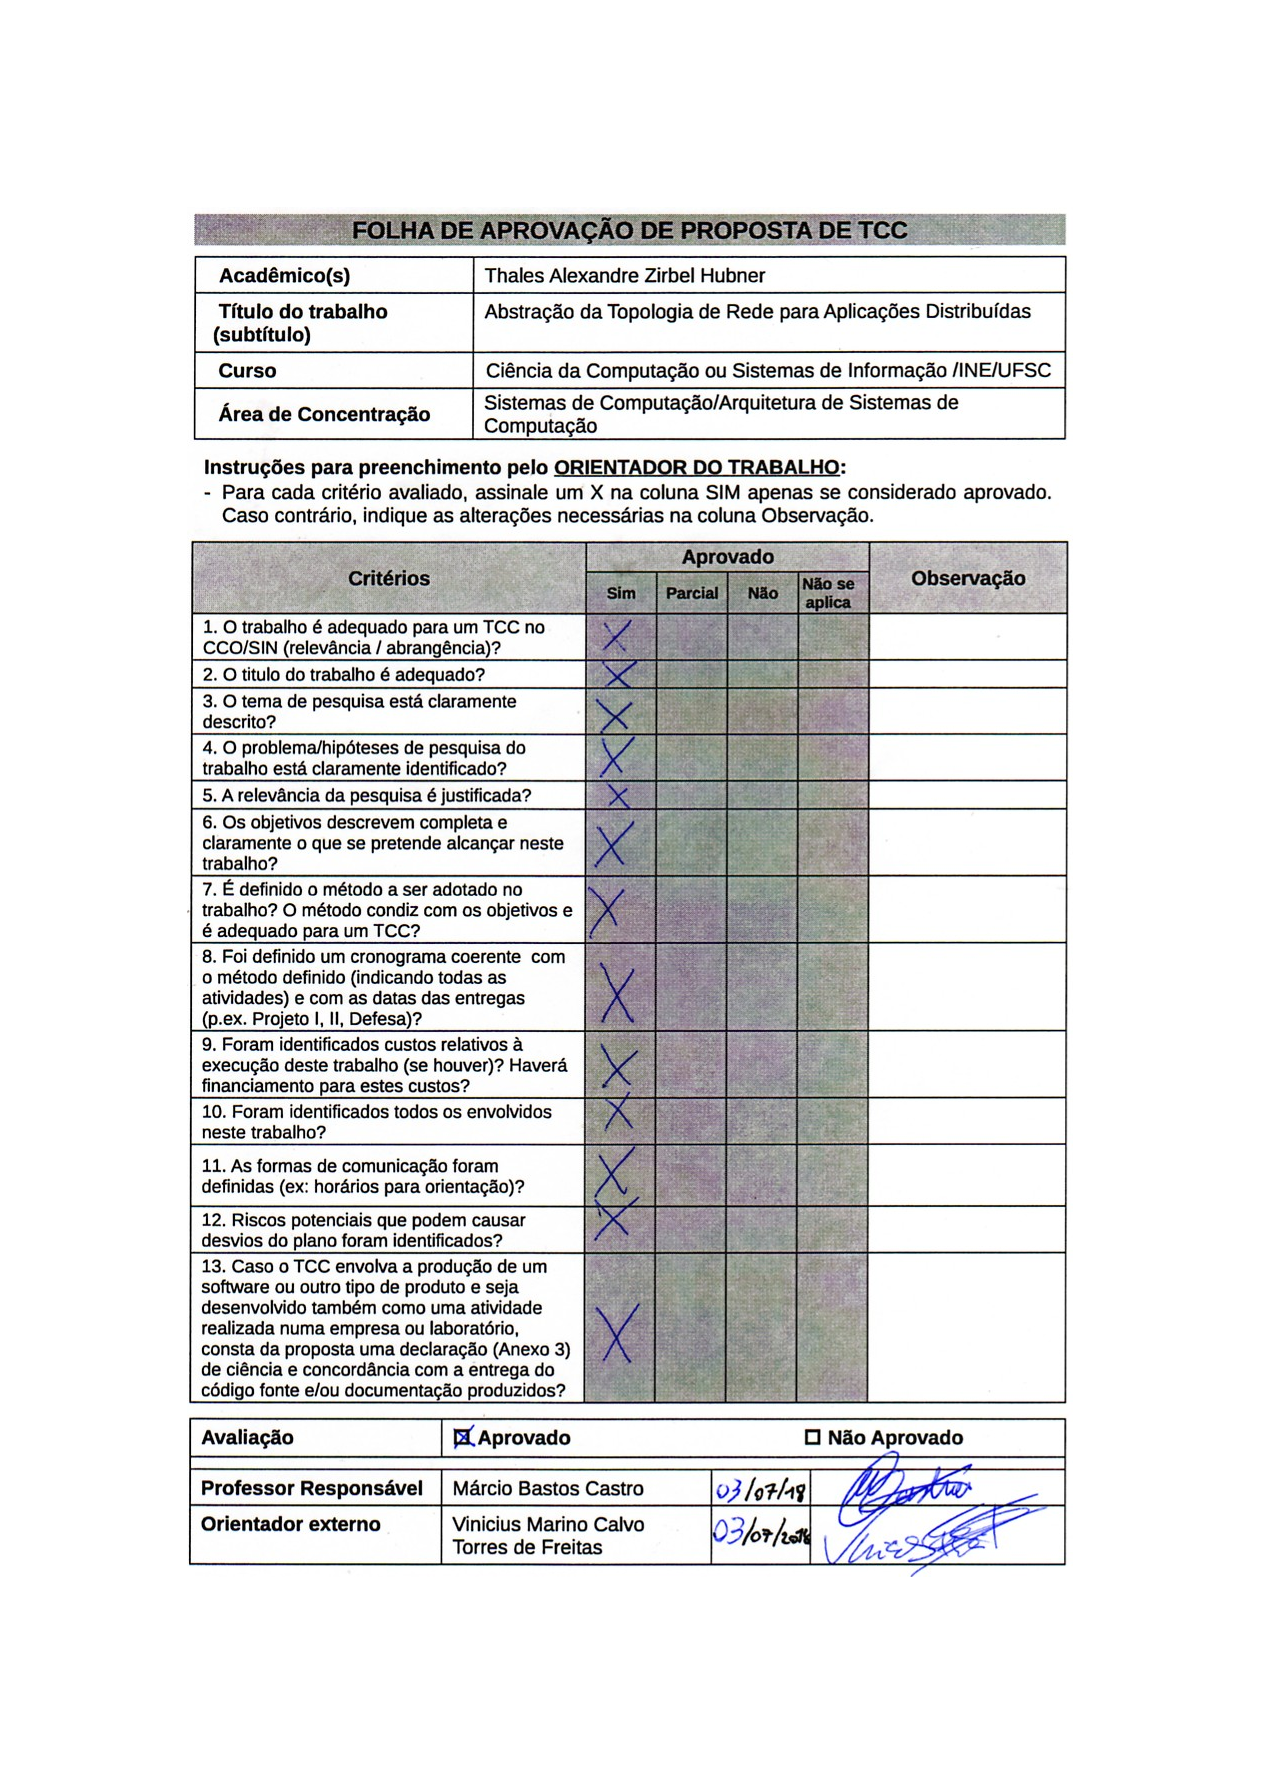
\includepdf{folha_aprovacao_assinada}  
%\end{folhadeaprovacao}
% ---

% ---
% RESUMOS
% ---

% resumo em português
\begin{resumo}

A repartição de trabalho em ambientes distribuídos é um problema relevante em aplicações como simulações sísmicas, dinâmica molecular e previsão de tempo pois estas possuem comportamento dinâmico, gerando desbalanceamento de carga no sistema. 
Uma das maneiras de resolver esse problema é a utilização de balanceadores de carga dinâmicos, cuja função é reduzir o tempo de execução da aplicação através de uma distribuição de tarefas mais homogênea. 
Uma alocação de tarefas que leva em consideração a topologia da rede pode reduzir latências de comunicação e efeitos e contenção alocando tarefas que se comunicam próximas uma da outra.
Entretanto, poucos balanceadores consideram a topologia do sistema de maneira dinâmica, devido à dificuldade do balanceador de obter informações de topologia de rede, como distância e proximidade de tarefas, e de levá-las em consideração para o remapeamento de tarefas.

Este trabalho visa a o desenvolvimento de uma abstração da topologia de rede, facilitando o acesso à informações de topologia mais complexas da rede e a utilização destas em aplicações distribuídas. 
Com base na modelagem proposta será modificado uma estratégia de balanceamento de carga ciente de topologia que utilizará esta abstração, comprovando seu funcionamento. 


%  Segundo a \citeonline[3.1-3.2]{NBR6028:2003}, o resumo deve ressaltar o
%  objetivo, o método, os resultados e as conclusões do documento. A ordem e a extensão
%  destes itens dependem do tipo de resumo (informativo ou indicativo) e do
%  tratamento que cada item recebe no documento original. O resumo deve ser
%  precedido da referência do documento, com exceção do resumo inserido no
%  próprio documento. (\ldots) As palavras-chave devem figurar logo abaixo do
%  resumo, antecedidas da expressão Palavras-chave:, separadas entre si por
%  ponto e finalizadas também por ponto.\citeonline{Emma}.\citeonline{Nielsen}.
%  \citeonline{Goodfellow-et-al-2016}

 \vspace{\onelineskip}
    
 \noindent
 \textbf{Palavras-chaves}: topologia de rede. balanceamento de carga. aplicações distribuidas. aplicações paralelas
 
\end{resumo}
\cleardoublepage

% resumo em inglês
% \begin{resumo}[Abstract]
%  \begin{otherlanguage*}{english}
%    This is the english abstract.

%    \vspace{\onelineskip}
 
%    \noindent 
%    \textbf{Key-words}: latex. abntex. text editoration.
%  \end{otherlanguage*}
% \end{resumo}

% ---
% inserir lista de ilustrações
% ---
\pdfbookmark[0]{\listfigurename}{lof}
\listoffigures*
\cleardoublepage
% ---

% ---
% inserir lista de tabelas
% ---
\pdfbookmark[0]{\listtablename}{lot}
\listoftables*
\cleardoublepage
% ---

% ---
% inserir lista de abreviaturas e siglas
% ---
\begin{siglas}
  \item[PE] \textit{Processing Element}, unidade de processamento
  \item[LB] \textit{Load Balancer}, balanceador de carga
  \item[hwloc] \textit{Portable Hardware Locality}
  \item[netloc] \textit{Portable Network Locality}
  \item[CSC] \textit{Compressed Sparse Columns}
\end{siglas}
% ---

% ---
% inserir lista de símbolos
% ---
\begin{simbolos}
    \item[$\textbf{S}$] Aceleração
    \item[$n$] Número de núcleos utilizados
    \item[$s$] Parcela paralelizável do programa
    \item[$d$] Número de dimensões da topologia
    \item[$k$] Número de nós por dimensão da topologia
    \item[$p$] Número de nós totais da topologia
    \item[$f$] Valor de \textit{fanout} da árvore
    \item[$h$] Número de \links remotos por roteador
    \item[$r$] Número de roteadores por grupo
    \item[$c$] Número de cores por máquina
    \item[$m$] Número de máquinas no sistema
%  \item[$ \Gamma $] Letra grega Gama
%  \item[$ \Lambda $] Lambda
%  \item[$ \zeta $] Letra grega minúscula zeta
%  \item[$ \in $] Pertence
\end{simbolos}
% ---

% ---
% inserir o sumario
% ---
\pdfbookmark[0]{\contentsname}{toc}
\tableofcontents*
\cleardoublepage
% ---



% ----------------------------------------------------------
% ELEMENTOS TEXTUAIS
% ----------------------------------------------------------
\textual


% ----------------------------------------------------------
% Introdução
% ----------------------------------------------------------
\chapter{Introdução}

Este capítulo apresenta o tema de pesquisa do Trabalho de Conclusão de Curso, o escopo no qual o problema em questão será tratado e a justificativa do projeto. Na Seção ~\ref{sec:introducao} é apresentado o contexto e a motivação para a realização do trabalho. Na Seção ~\ref{sec:objetivos} são introduzidos os objetivos gerais e específicos, as restrições e premissas existentes, a lista de marcos e os critérios de aceite do projeto. Na Seção ~\ref{sec:metodologia}, são abordados os métodos de pesquisa envolvidos para alcançar a solução proposta.


\section{Motivação}
\label{sec:introducao}

Aplicações no âmbito científico e industrial incluem cada vez mais detalhes, demandam precisão ainda maior e/ou possuem uma complexidade muito elevada, criando uma demanda cada vez maior por velocidade e poder de processamento~\cite{pilla-thesis}. Uma das maneiras utilizadas para suprir esta demanda é com computação paralela, que alcança a solução destes problemas através da repartição de trabalho entre unidades de processamento (\textit{Processing Elements} ou PEs) e a execução destas parcelas simultaneamente. Este método permite que um aumento no número de PEs leve a uma redução no tempo da aplicação. Contudo a melhoria no tempo é limitada pela parcela não paralelizável do programa e pelos recursos do sistema~\cite{amdahl}. 

Supercomputadores que utilizam da computação paralela foram criados para alcançar processamento massivo e por décadas estas máquinas cresceram. Elas alcançaram um ponto onde se percebeu que velocidade e poder de processamento não eram as métricas adequadas para desempenho destas máquinas. Estes computadores consomem uma quantidade tremenda de energia que é em maior parte dissipada, se transformando em grandes geradores de calor~\cite{green500}. A geração de calor excessiva é um problema em sistema pois temperaturas altas aumentam sua chance de falha e tempo fora de operação~\cite{efficient-metric}. Como contramedida é necessário a implantação de um sistema eficiente de redução de temperatura, que traz outro grande sobrecusto de energia. Com estes problemas em mente a métrica pensada para estas máquinas é a eficiência de processamento, que leva em conta a energia gasta no sistema, a velocidade e o poder de processamento~\cite{efficient-metric}.

Uma das opções para obter eficiência de processamento é o uso de um número maior de núcleos menos potentes~\cite{snir-encyclopedia}. A organização de um número grande de PEs acaba levando a um sistema com memória distribuída, que operam com o uso de diversas máquinas e utilizam alguma rede para a interligação e comunicação. A escolha destes sistemas é devida ao seu custo baixo e a sua grande escalabilidade através do aumento no número de máquinas. O contraponto destas vantagens é o desenvolvimento destas aplicações, que se torna mais complexo pois têm de levar em consideração fatores impactantes como sincronização, dependência e distribuição de dados, balanceamento de carga e custos de comunicação~\cite{pilla-thesis}.

A comunicação em um sistema distribuído é realizado através de \links de conexão que ligam PEs. Estas ligações estão dispostas utilizando algum padrão de topologia, como malhas, tori \fatts ou \dgfly, que buscam otimizar alguma característica da rede, como custo de implantação, tráfego ou latência média. A alocação de tarefas nestes sistemas geralmente ocasiona um uso compartilhado de \links por múltiplos núcleos, que pode saturar partes da rede devido a uma carga maior de informação a ser transmitida do que os \links suportam, resultando em contenção~\cite{bhatele-encyclopedia}. Outro fator de topologia que impacta o desempenho da aplicação é a possibilidade da rede ter ligações com custos heterogêneos~\cite{dragonfly}, tendo latências diferentes para \links diferentes.

%old:  Os PEs em sistemas distribuídos se comunicam usando diversas topologias de rede, como malhas, tori, \fatts ou \dgfly. Os núcleos utilizam de \textit{links} de conexão da rede para efetuar comunicação no sistema. O compartilhamento destes pode resultar em congestão, um congestionamento da rede devido ao sobreuso de alguns \links~\cite{bhatele-encyclopedia}. Outro fator é a possibilidade da rede não ter ligações com custos iguais de comunicação~\cite{dragonfly}, tendo variações de latência e velocidade em partes distintas da rede. O impacto disto é que os caminhos menos custosos entre PEs na rede nem sempre são os menores em questão de \links percorridos.

A repartição de trabalho em ambientes distribuídos é um problema a ser tratado, pois aplicações como simulações sísmicas~\cite{dupros}~\cite{tesser}, dinâmica molecular~\cite{bhatele-kale} ou previsão de tempo~\cite{rodrigues} possuem comportamento dinâmico, ou seja suas cargas mudam ao longo da execução da aplicação, levando um mapeamento homogêneo de tarefas a um estado desbalanceado do sistema, resultando em uma diferença de carga entre alguns PEs. Esta diferença faz com que alguns PEs não tenham trabalho para executar enquanto esperam a conclusão de tarefas nos PEs mais carregados, reduzindo o desempenho geral da aplicação. Para consertar tais desvios pode-se usar um balanceador de carga (\textit{Load Balancer} ou LB) dinâmico, cujo trabalho é remapear as tarefas entre os PEs, buscando um estado mais balanceado do sistema. Este rearranjo garante a utilização dos PEs de maneira mais homogênea e leva a uma redução do tempo da aplicação pela redução de tempo ocioso.

Os caminhos utilizados dentro de uma rede impactam o tempo de execução de um programa, pois caminhos mais lentos resultam em uma latência maior de comunicação e problemas como contenção podem ocorrer. É possível que aplicações e LBs levem em conta os custos de comunicação entre os PEs e os custos de movimentação destas tarefas dentro da rede. Tal abordagem pode levar a uma redução do custo de comunicação, evitando a troca de informação e tarefas através de partes lentas da rede. Uma abstração da topologia de rede que permita fácil acesso as informações da rede e de comunicação reduziria a complexidade de criação de aplicações que levem em conta estes problemas.
% olhar netloc para referencia

\section{Objetivos}
\label{sec:objetivos}

Os objetivos deste trabalho são de desenvolver e avaliar uma abstração da topologia de rede, permitindo seu uso para balanceadores de carga e aplicações distribuídas. Para este fim, seguem os objetivos específicos:

\begin{enumerate}
\item Desenvolver uma API de acesso à informações de topologia de rede;
\item Implementar algoritmos e estruturas para o uso destas informações;
\item Desenvolver uma interface desta abstração utilizando a plataforma Charm++~\cite{website:CHARM};
\item Desenvolver um LB que utilize esta base, visando a prova funcional da abstração.

\end{enumerate}

\begin{flushleft}
\textbf{Premissas:}
\begin{itemize}
\item Um computador estará disponível para realização do trabalho; 
\item O orientador terá disponibilidade para reuniões periódicas;
\item Disponibilidade de energia e internet.
\item Acesso a uma máquina com uma topologia diferenciada para a realização dos testes.
\end{itemize}

\textbf{Marcos:}
\begin{itemize}
 
\item Entrega do resumo em TCC I: 4ª semana de Novembro/2018; 
\item Entrega da abstração implementada: 4ª semana de Janeiro/2018;
\item Entrega da interface com \charm: 1ª semana de Abril/2019;
\item Entrega do Balanceador modificado: 4ª semana de Abril/2019;
\item Entrega da primeira versão da monografia em TCC II: 2ª semana de Maio/2019; 
\item Defesa da monografia: 2ª semana de Junho/2019;
\item Entrega da versão final da monografia em TCC II: 4ª semana de Junho/2019.
\end{itemize}

\textbf{Critérios de aceite:}
\begin{itemize}
\item Aprovação da banca avaliadora;
\item Aprovação do orientador;
\item Aprovação do coorientador;
\item Conformidade da monografia com as normas definidas pela instituição;
\item Prazos cumpridos.
\end{itemize}
\end{flushleft}

\section{Método de Pesquisa}
\label{sec:metodologia}

 
O início do trabalho teve duas partes: uma de cunho teórico, onde foi estudado os conceitos de e o estado da arte para o projeto, e outra mais prática, que envolveu o aprendizado do \textit{framework} \charm. A primeira parcela foi constituída por um estudo sobre topologia de rede e balanceamento de carga em aplicações paralelas, criando uma base de conhecimentos para o projeto. A segunda parte teve foco no entendimento da plataforma e suas nuances, visando facilitar a implementação da abstração.

A criação da abstração da topologia de rede utilizará a linguagem de programação C++ e será posteriormente inicializada com informações do \fw de programação paralela \charm~\cite{website:CHARM}. Essa plataforma será utilizada pois têm uma base sólida para a criação, utilização e teste de balanceadores de carga e outras aplicações paralelas~\cite{bhatele-thesis}. Além disto, \charm contém somente abstrações de topologia fixas (detalhado na seção~\ref{sec:charm}), carecendo de uma abstração elaborada da topologia de rede, proposta neste trabalho.

Para a criação da abstração de topologia de rede, foi criada uma especificação de suas funções e suas estruturas, criando um esqueleto que pode ser preenchido posteriormente. Um estudo de estruturas e algoritmos utilizados no estado da arte será realizada para observar como tais funções podem ser implementadas de maneira eficiente.

Após a implementação dos algoritmos e estruturas da abstração de topologia de rede será implementado um método de inicialização da estrutura através do \fw \xspace \charm, que coleta as informações necessárias para a execução de seu \textit{runtime} que podem ser utilizadas na abstração.

Na última etapa do projeto será modificado um balanceador de carga ciente de topologia para utilizar esta abstração de rede, demonstrando seu funcionamento e sua utilidade através das funções implementadas e utilizadas, e então comparado com o original, buscando verificar seu sobrecusto.

% Após a criação e teste da abstração da topologia de rede, será desenvolvido um LB que utiliza desta abstração para reduzir o custo de comunicação dentro de uma rede com custos de comunicação heterogêneos. O balanceador também será realizado em C++ na plataforma \charm. Serão executados testes de funcionamento e avaliação de desempenho.

% Na última etapa será realizado uma análise de desempenho do LB em comparação com outros LB's, verificando sua efetividade e seu sobrecusto como balanceador de carga. Para tal, serão realizados experimentos utilizando algum \textit{benchmark} que simule aplicações reais. O teste será realizado em um cenário onde a topologia tem custos de comunicação heterogêneos e outra com custos homogêneos. Também será realizado um teste para verificar o sobrecusto do LB em um cenário onde não há benefícios em balanceamento de carga.


% ----------------------------------------------------------
% PARTE - preparação da pesquisa
% ----------------------------------------------------------
% \part{Preparação da pesquisa}

% ----------------------------------------------------------
% Capitulo com exemplos de comandos inseridos de arquivo externo 
% ----------------------------------------------------------

\include{abntex2-modelo-include-comandos}

% ----------------------------------------------------------
% Parte de revisão de literatura
% ----------------------------------------------------------
% \part{Revisão de Literatura}

% ---
% Capitulo de revisão de literatura
% ---
\chapter{Fundamentação Teórica}

O desempenho de um aplicação paralela depende de uma multitude de fatores como \textit{hardware}, técnicas de otimização, topologia, arquitetura utilizada, políticas tomadas e comunicação. Na Seção~\ref{sec:parellel} são abordados questões de computação paralela, incluindo algumas de suas características e alguns de seus limites. A Seção~\ref{sec:topologia} aborda topologias de sistemas paralelos, suas características e seu impacto na aplicação. Na Seção~\ref{sec:lb} é tratado o que é um balanceador de carga, que problemas um estes buscam resolver e os benefícios de um balanceador ciente de topologia.


\section{Computação Paralela}
\label{sec:parellel}

Uma aplicação paralela realiza computação de maneira concorrente, utilizando os recursos de processamento disponíveis simultaneamente para a realização destas tarefas. O ganho de desempenho ao se realizar coisas simultaneamente é pago com uma complexidade maior de \textit{hardware}, arquiteturas e com a necessidade de sincronização, garantias de exclusão, trocas de mensagem e outras técnicas de programação e compilação~\cite{david-encyclopedia}.

O fim da lei de moore~\cite{patterson} e o limite da barreira de potência tornou a redução dos transistores e o aumento na frequência dos processadores insuficiente, abrindo um espaço para os ganhos de arquiteturas paralelas~\cite{tanenbaum:operational_systems}. Em ambientes de múltiplos núcleos se utiliza um número maior de núcleos menos poderosos, em busca de eficiência através de um paralelismo maior e de um consumo de energia mais baixo~\cite{snir-encyclopedia}. Estes sistemas são facilmente escalados através da inclusão de mais núcleos e extensão da rede, mas agregam uma série de complexidades para o desenvolvimento devido à dimensão a mais, como sincronização, dependência e distribuição de dados, balanceamento de carga e custos de comunicação entre os núcleos~\cite{pilla-thesis}.

A relação entre a aceleração de uma aplicação $(\textbf{S})$ com o número de núcleos utilizados ($n$) e sua parcela paralelizável ($s$) é expressa pelo argumento de Amdahl na Equação~\ref{eq:amdahl}~\cite{amdahl}. A fórmula segue abaixo, representada como a Equação~\ref{eq:amdahl}. É importante constatar que são desconsiderados detalhes como os custos de acesso a memória, envio de mensagens, geração de \textit{threads} e latência de interconexão. A fórmula é então utilizada como uma estimativa para a aceleração e não como uma referência exata, pois o impacto exato não é simples de calcular.

\begin{equation}
\textit{\textbf{S}} = \frac{1}{(1-\textit{s}) + \frac{\textit{s}}{\textit{n}}}
\label{eq:amdahl}
\end{equation}

Na Equação~\ref{eq:amdahl}, quando $c$ tende ao infinito a equação indica um limite na aceleração de acordo com a parcela serial do programa $(1-s)$, pois esta não se beneficia da paralelização. 
Levando este limite em conta, as aplicações paralelas muitas vezes são adaptadas para que sua parte paralelizável inclua mais detalhes ou mais precisão, fazendo com que um aumento no número de PEs leve à mais informação sendo processada e não à uma aceleração~\cite{gustafson}.

\subsection{Carga e Comunicação}

O processamento a ser realizado em uma aplicação paralela é dividido em tarefas e em cargas. 
A carga representa a quantidade de processamento que uma tarefa precisa realizar em um único PE. 
Em um sistema paralelo, múltiplas tarefas são executadas concorrentemente, tendo sua carga distribuída entre os PEs do sistema. 
Um núcleo que possui uma carga maior que um limiar acima da média é considerado sobrecarregado, e um núcleo que tem menos carga que um limiar abaixo da media é considerado subcarregado. 
Esta diferença nas cargas faz com que alguns PEs não tenham trabalho para executar enquanto esperam a conclusão de tarefas nos PEs mais carregados, sub-utilizando o sistema. 
Esta situação é chamada de desbalanceamento.

\begin{figure} [b]
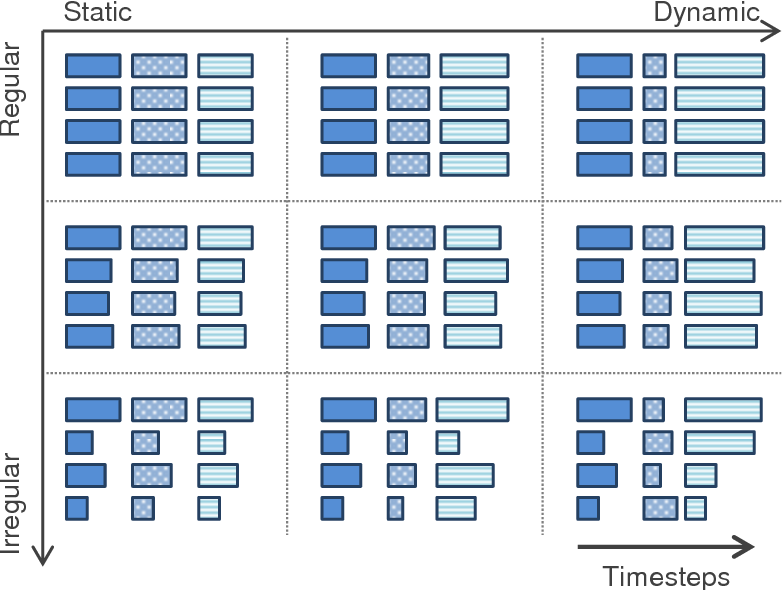
\includegraphics[width=0.62\textwidth]{load_pilla}
\centering
\caption[Diferentes graus de regularidade e dinamicidade em relação a carga de uma aplicação.]{Diferentes graus de regularidade e dinamicidade em relação a carga de uma aplicação ~\cite{pilla-thesis}.}
\label{fig:load}
\end{figure}

Em aplicações paralelas a carga de uma tarefa e sua comunicação podem ser diferentes da a de outras tarefas ou podem variar ao longo do tempo. 
Duas características refletem isso: a Regularidade e a Dinamicidade. 
A regularidade de uma aplicação reflete o quanto a carga ou a comunicação de uma tarefa difere de uma outra tarefa. Uma aplicação com carga ou comunicação regular têm cargas ou comunicação aproximadamente iguais. 
Quanto a carga ou comunicação difere entre tarefas, a aplicação têm carga ou comunicação irregular, respectivamente.
A dinamicidade de uma aplicação indica o quanto a comunicação ou carga de uma tarefa muda ao longo do tempo. Quando sua carga ou comunicação não muda ao longo do tempo, é dita estática e quando muda, é dita dinâmica~\cite{pilla-thesis}.
As Figuras~\ref{fig:load} e \ref{fig:communication} apresentam a variação de regularidade e dinamicidade em relação a carga e a comunicação de uma tarefa, respectivamente. 

\begin{figure} [h]
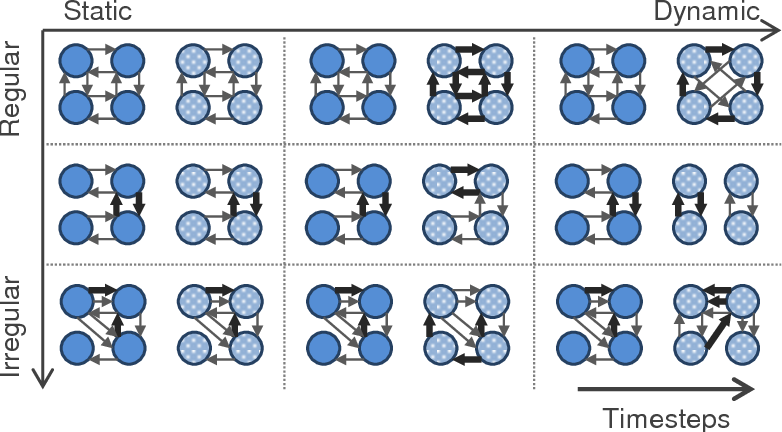
\includegraphics[width=0.67\textwidth]{comm_pilla}
\centering
\caption[Diferentes graus de regularidade e dinamicidade em relação a comunicação de uma aplicação.]{Diferentes graus de regularidade e dinamicidade em relação a comunicação de uma aplicação ~\cite{pilla-thesis}.}
\label{fig:communication}
\end{figure}

A distribuição de tarefas em um ambiente paralelo deve levar em consideração sua regularidade e dinamicidade. 
Técnicas de escalonamento, alocação de tarefas e balanceamento de carga são utilizadas para gerenciar e dispor as tarefas de maneira eficiente no sistema. 
Na Seção~\ref{sec:lb} é detalhado uma destas técnicas, a de balanceamento de carga.

\subsection{Computação distribuída}

Em ambientes multiprocessados, existe algum dispositivo de memória compartilhada entre todos os PEs que é organizada para que problemas de coerência e consistência não ocorram. 
Chips \textit{multicore} e \textit{manycore} são exemplos de ambientes multiprocessados. 
Ambientes multiprocessados não escalam bem devido a complexidade de arquitetura e custos de produção, abrindo espaço para ambientes multicomputados. 
Em ambientes multicomputados a memoria não é compartilhada entre todos os PEs e algum meio de interconexão é utilizado para realizar as trocas de informação, mas o sistema ainda é organizado de maneira similar~\cite{tanenbaum:operational_systems}.

Em um sistema distribuído, computadores com diferentes arquiteturas, organizações, locais e comportamentos podem ser interconectados em uma mesma rede e utilizados em conjunto. 
Devido a alta independência dos componentes, estes sistemas são altamente escaláveis através da adição de computadores e expansão da rede. 
A comunicação e coordenação destes sistemas se torna muito mais complexa e custosa~\cite{tanenbaum:operational_systems}.


\section{Topologia de rede}
\label{sec:topologia}

Sistemas paralelos utilizam redes de interconexão para efetuar a comunicação entre seus PEs. 
Estas redes têm propriedades como diâmetro, distância média, grau, latências e largura de banda que regem a comunicação dentro da rede. 
O padrão de interconexões entre PEs é chamado de topologia e esta pode assumir diversas formas como malhas, tori e \textit{fat-trees}.

As topologias de uma rede podem ser dividas em duas categorias: diretas e indiretas. 
Em redes diretas, cada PE é conectado diretamente com outro processador com um \link e para uma mensagem ir de uma fonte a um destino, ela cruza vários destes \links.
O cruzamento de um \link é chamado de \hop e a distância entre um ponto a outro na rede pode ser definido pelo número de \hops realizados. 
Malhas, tori e hipercubos são exemplos de redes diretas. 
Em redes indiretas, PEs são conectados a \switches que roteiam as mensagens. Nenhum PE é ligado diretamente a outro PE e portanto é necessário cruzar dois ou mais \switches para alcançar outro PE. 
\Fatts e \dgfly são exemplos de redes indiretas~\cite{bhatele-encyclopedia}.

A hierarquia é um fator presente em algumas topologias indiretas, como \fatt e \dgfly, e divide esta em níveis de proximidade. 
Cada nível de hierarquia na topologia representa um agrupamento diferente da rede. 
Redes hierárquicas apresentam pontos de gargalo de tráfego entre seus níveis e requerem uma replicação de \links para que isto não se torne um problema.

Uma rede de interconexão tem duas propriedades importantes que afetam sua comunicação: Simetria e Uniformidade. 
Um nível de topologia é dito simétrico quando o tempo de comunicação de um ponto A para um ponto B é o mesmo que de B para A e é dito assimétrico quando isto não ocorre. 
Um nível de topologia é uniforme quando todos os PEs neste nível tem o mesmo tempo de comunicação entre si~\cite{pilla-thesis}. 
Uma rede indireta pode se tornar assimétrica devido ao roteamento de informações. 
%problema: parece estar mal formulado e estranho porque por exemplo de p1 a p3 pode ter um caminho mais longo (tori por exemplo)
%problema tem alguma utilidade falar isso?

\begin{figure} [b]
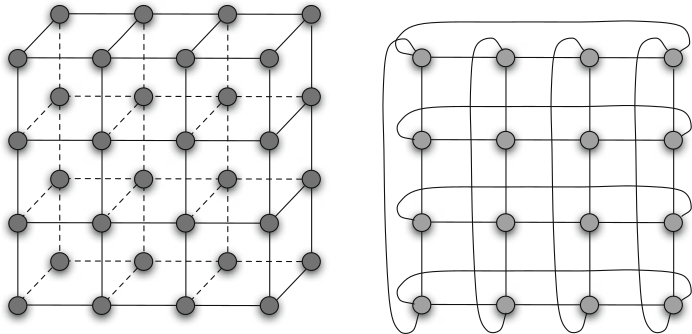
\includegraphics[width=0.5\textwidth]{mesh_torus}
\centering
\caption[Uma malha de dimensões (4,4,2) e uma torus 2D]{Uma malha de dimensões (4,4,2) a esquerda e uma torus 2D a direita~\cite{bhatele-encyclopedia}}
\label{fig:mesh_torus}
\end{figure}

Algumas métricas são utilizadas para observar o comportamento de uma rede, como o diâmetro, o número de \links, o grau e a bisseção de \links. 
O diâmetro de uma rede é definida como sendo o maior caminho dentre os caminhos mais curtos que ligam quaisquer dois nós da topologia, é medida através de \hops e é uma utilizada para ver qual é o pior caso de distância na rede e portanto a maior latência dentro da rede. 
O número de \links apresenta a quantidade total de \links dentro da rede, uma informação usada para avaliar o custo de implantação. 
O grau de uma rede é o número de \links conectados em cada nó da rede. 
A bisseção da largura de banda representa a quantidade de \links entre duas partes da rede, partida de modo a gerar o mínimo de \links entre duas metades da rede. 
Essa métrica e utilizada para estimar o quanto de tráfego a rede suporta~\cite{david:paralel}. 
Em sequência seguem algumas topologias abordadas ao longo da seção.

\begin{figure} [t]
    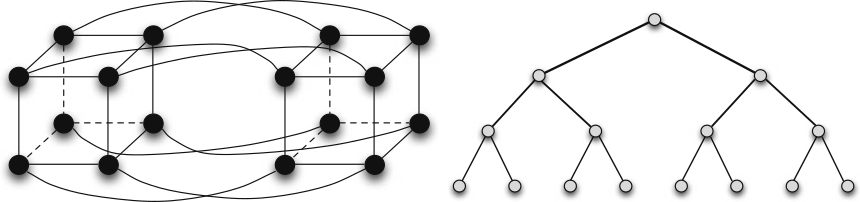
\includegraphics[width=0.7\textwidth]{hypercube_fat_tree}
    \centering
    \caption[Um hipercubo de e uma \fatt]{Uma rede direta em forma de hipercubo de 4 dimensões a direita e uma indireta em forma de \fatt binária com 4 níveis a esquerda~\cite{bhatele-encyclopedia}}
    \label{fig:cube_fat}
\end{figure}

\begin{itemize}
    \item \textbf{Malha}: Uma topologia direta similar a uma matriz de múltiplas dimensões, onde cada \link só cruza uma dimensão da rede e na menor distância possível ~\cite{Solihin}.
    Malhas podem ser dispostas em diversas dimensões, na Figura~\ref{fig:mesh_torus} é representada uma malha de dimensões 4, 4 e 2.
    
    \item \textbf{Torus}: Uma malha com um \link entre nodos finais de cada dimensão da rede, reduzindo o diâmetro da rede e aumentando sua bisseção. 
    Uma torus de dimensões 4 e 4 pode ser observada na Figura~\ref{fig:mesh_torus}
    
    \item \textbf{Hipercubo}: Uma malha com 2 nodos em cada dimensão.
    Um hipercubo visa reduzir a distancia máxima da rede. 
    A Figura~\ref{fig:cube_fat} mostra um exemplo de hipercubo.
    
    \item \textbf{\Fatt}: Uma topologia de rede indireta em forma de árvore, onde \links em níveis mais altos tenham mais largura de banda. 
    Esta topologia é encontrada como topologia interna de máquinas. 
    Uma \fatt é representada na Figura~\ref{fig:cube_fat}.
    
    \item \textbf{\textit{Butterfly}}: Uma topologia indireta que visa escalabilidade e redução de distâncias através da replicabilidade de \links e de roteadores.
    É utilizada para gerar superconexão em uma rede.
    Seu problema é devido ao grande número de \links, que é muito superior as outras topologias~\cite{david:paralel}.
    
    \item \textbf{\Dgfly}: Uma topologia indireta que cria agrupamentos de roteadores em grupos distintos, visando reduzir o número de \links da rede para reduzir seu custo.
    Será tratada com mais detalhe na Seção~\ref{sec:dgfly} por possuir algumas características de topologia relevantes para a alocação de tarefas.
\end{itemize}

\begin{figure} [h]
    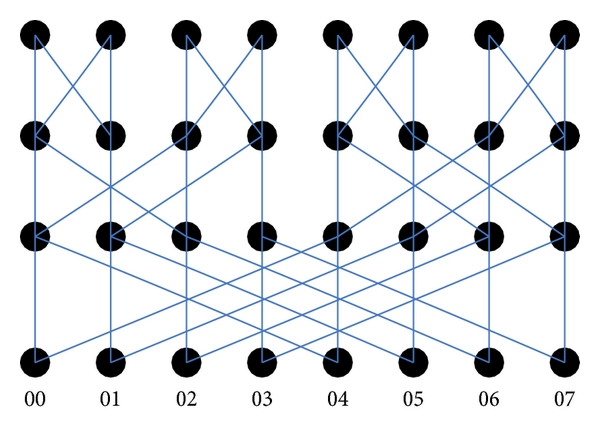
\includegraphics[width=0.4\textwidth]{bfly}
    \centering
    \caption[Uma rede \textit{Buttefly}]{Uma rede \textit{butterfly} de 3 níveis e 8 nós~\cite{Liu:bfly}}
    \label{fig:bfly}
\end{figure}

\setlength{\tabcolsep}{0.5em}
\begin{table}[h]
    \centering
    \begin{tabular}{c l}
        \toprule
        \textbf{Símbolo} &    \textbf{Descrição}  \\ \midrule
        $d$ & Número de dimensões da topologia.  \\ %\hline
        $k$ & Número de nós por dimensão da topologia.  \\ %\hline
        $p$ & Número de nós totais da topologia.  \\ %\hline
        $f$ & Valor de \textit{fanout} da árvore.  \\ %\hline
        $h$ & Número de \links remotos por roteador \\ %\hline
        $r$ & Número de roteadores por grupo \\ \bottomrule
    \end{tabular}
    \caption[Símbolos utilizados na Tabela~\ref{tab:topo_comparison}]{Símbolos utilizados na Tabela~\ref{tab:topo_comparison}.}
    \label{tab:topo_symbols}
\end{table}

\setlength{\tabcolsep}{0.5em}
\begin{table}[!h]
    \centering
    \begin{tabular}{l c c c c}
        \toprule
        \textbf{Topologia} &    \textbf{Diâmetro} &  \textbf{Bisseção} &   \textbf{\Links} &     \textbf{Grau} \\ \midrule
        Malha & $dk-1$ & $k^{d-1}$ &   $dk^{d-1} \times (k-1)$ &    $2d$  \\ %\hline
        Tori  & $\frac{dk}{2}-1$ & $k^d$ & $dk^d$ &  $2d$  \\ %\hline
        Hipercubo &  $\log_2 p$ & $\frac{p}{2}$ &  $log_2 p \times \frac{p}{2}$  &  $\log_2 p$  \\ %\hline
        \Fatt &  $2 \times \log_f p$ & $\frac{p}{2}$ & $f(p-1)$ &  $f + 1$  \\ %\hline
        \textit{Butterfly} & $\log_2 p$ & $\frac{p}{2}$ &  $2p \times \log_2 p$ &  $4$  \\ %\hline
        \Dgfly & $3$  & $h((r+2)^2/4) $  &  $ r\times(r-1) +rh  $ & $r + h$ \\\bottomrule
    \end{tabular}
    \caption[Diâmetro, bisseção de \links, número \links e grau das topologias de Malha, Tori, Hipercubo, \Fatt, \textit{Butterfly} e \Dgfly.]{Diâmetro, bisseção de \links, número de \links e grau das topologias Malha, Tori, Hipercubo, \Fatt, \textit{Butterfly} e \Dgfly~\cite{li:dgfly}. Os símbolos utilizados são apresentados na Tabela~\ref{tab:topo_symbols}. Adaptado de ~\cite{Solihin}.}
    \label{tab:topo_comparison}
\end{table}

A Tabela~\ref{tab:topo_comparison} apresenta algumas topologias e seu comportamento em relação a diâmetro, bisseção, \links e grau. Os símbolos utilizados são descritos na Tabela~\ref{tab:topo_symbols}.
É importante ressaltar que $p = dk$ nas topologias de Malha ou Tori.
Na Tabela~\ref{tab:topo_example} são comparadas topologias com $2^{16}$ nós.
A topologia \dgfly se destaca pois têm \links com latências diferentes e custos de implementação diferentes, fazendo com que métricas baseadas em \hops e número de \links não reflitam a distância e o desempenho da rede.


\setlength{\tabcolsep}{0.5em}
\begin{table}[!ht]
    \centering
    \begin{tabular}{l c c c c}
        \toprule
        \textbf{Topologia} &    \textbf{Diâmetro} &  \textbf{Bisseção} &   \textbf{\Links} &     \textbf{Grau} \\ \midrule
        Malha 4D & $63$ & $4096$ & $245760$ &  $8$  \\ %\hline
        Tori 4D & $31$ & $65536$ & $262143$ &  $8$  \\ %\hline
        Hipercubo &  $16$ & $32768$ &  $524288$  &  $16$  \\ %\hline
        \Fatt &  $16$ & $32768$ & $262143$ &  5  \\ %\hline
        \textit{Butterfly} & $16$ & $32768$ &  $2097152$ &  $4$  \\ %\hline
        \Dgfly & $3$  & $4225$  &  $ 16896 $ & $129$ \\ \bottomrule
    \end{tabular}
    \caption[Diâmetro, bisseção de banda, número de \links e grau das topologias com 64000 nodos.]{Diâmetro, bisseção de banda, número de \links e grau das topologias de Malha 4D, Tori 4D, Hipercubo, \Fatt de \textit{fanout} 4, \textit{Butterfly} e \Dgfly, todas com $2^{16}$ (65536) nodos.}
    \label{tab:topo_example}
\end{table}


Conforme cresce o número de PEs de um sistema, o fluxo de informação na rede aumenta e mais recursos de rede (\links e \switches) são compartilhados e disputados pelos PEs.
Este compartilhamento pode levar a um problema chamado de contenção, onde a latência da rede aumenta devido a saturação dos \links.
Um mapeamento de tarefas ciente de topologia de rede pode reduzir o compartilhamento de recursos de rede e portanto melhorar o desempenho da aplicação~\cite{bhatele-encyclopedia}.

\begin{figure} [h]
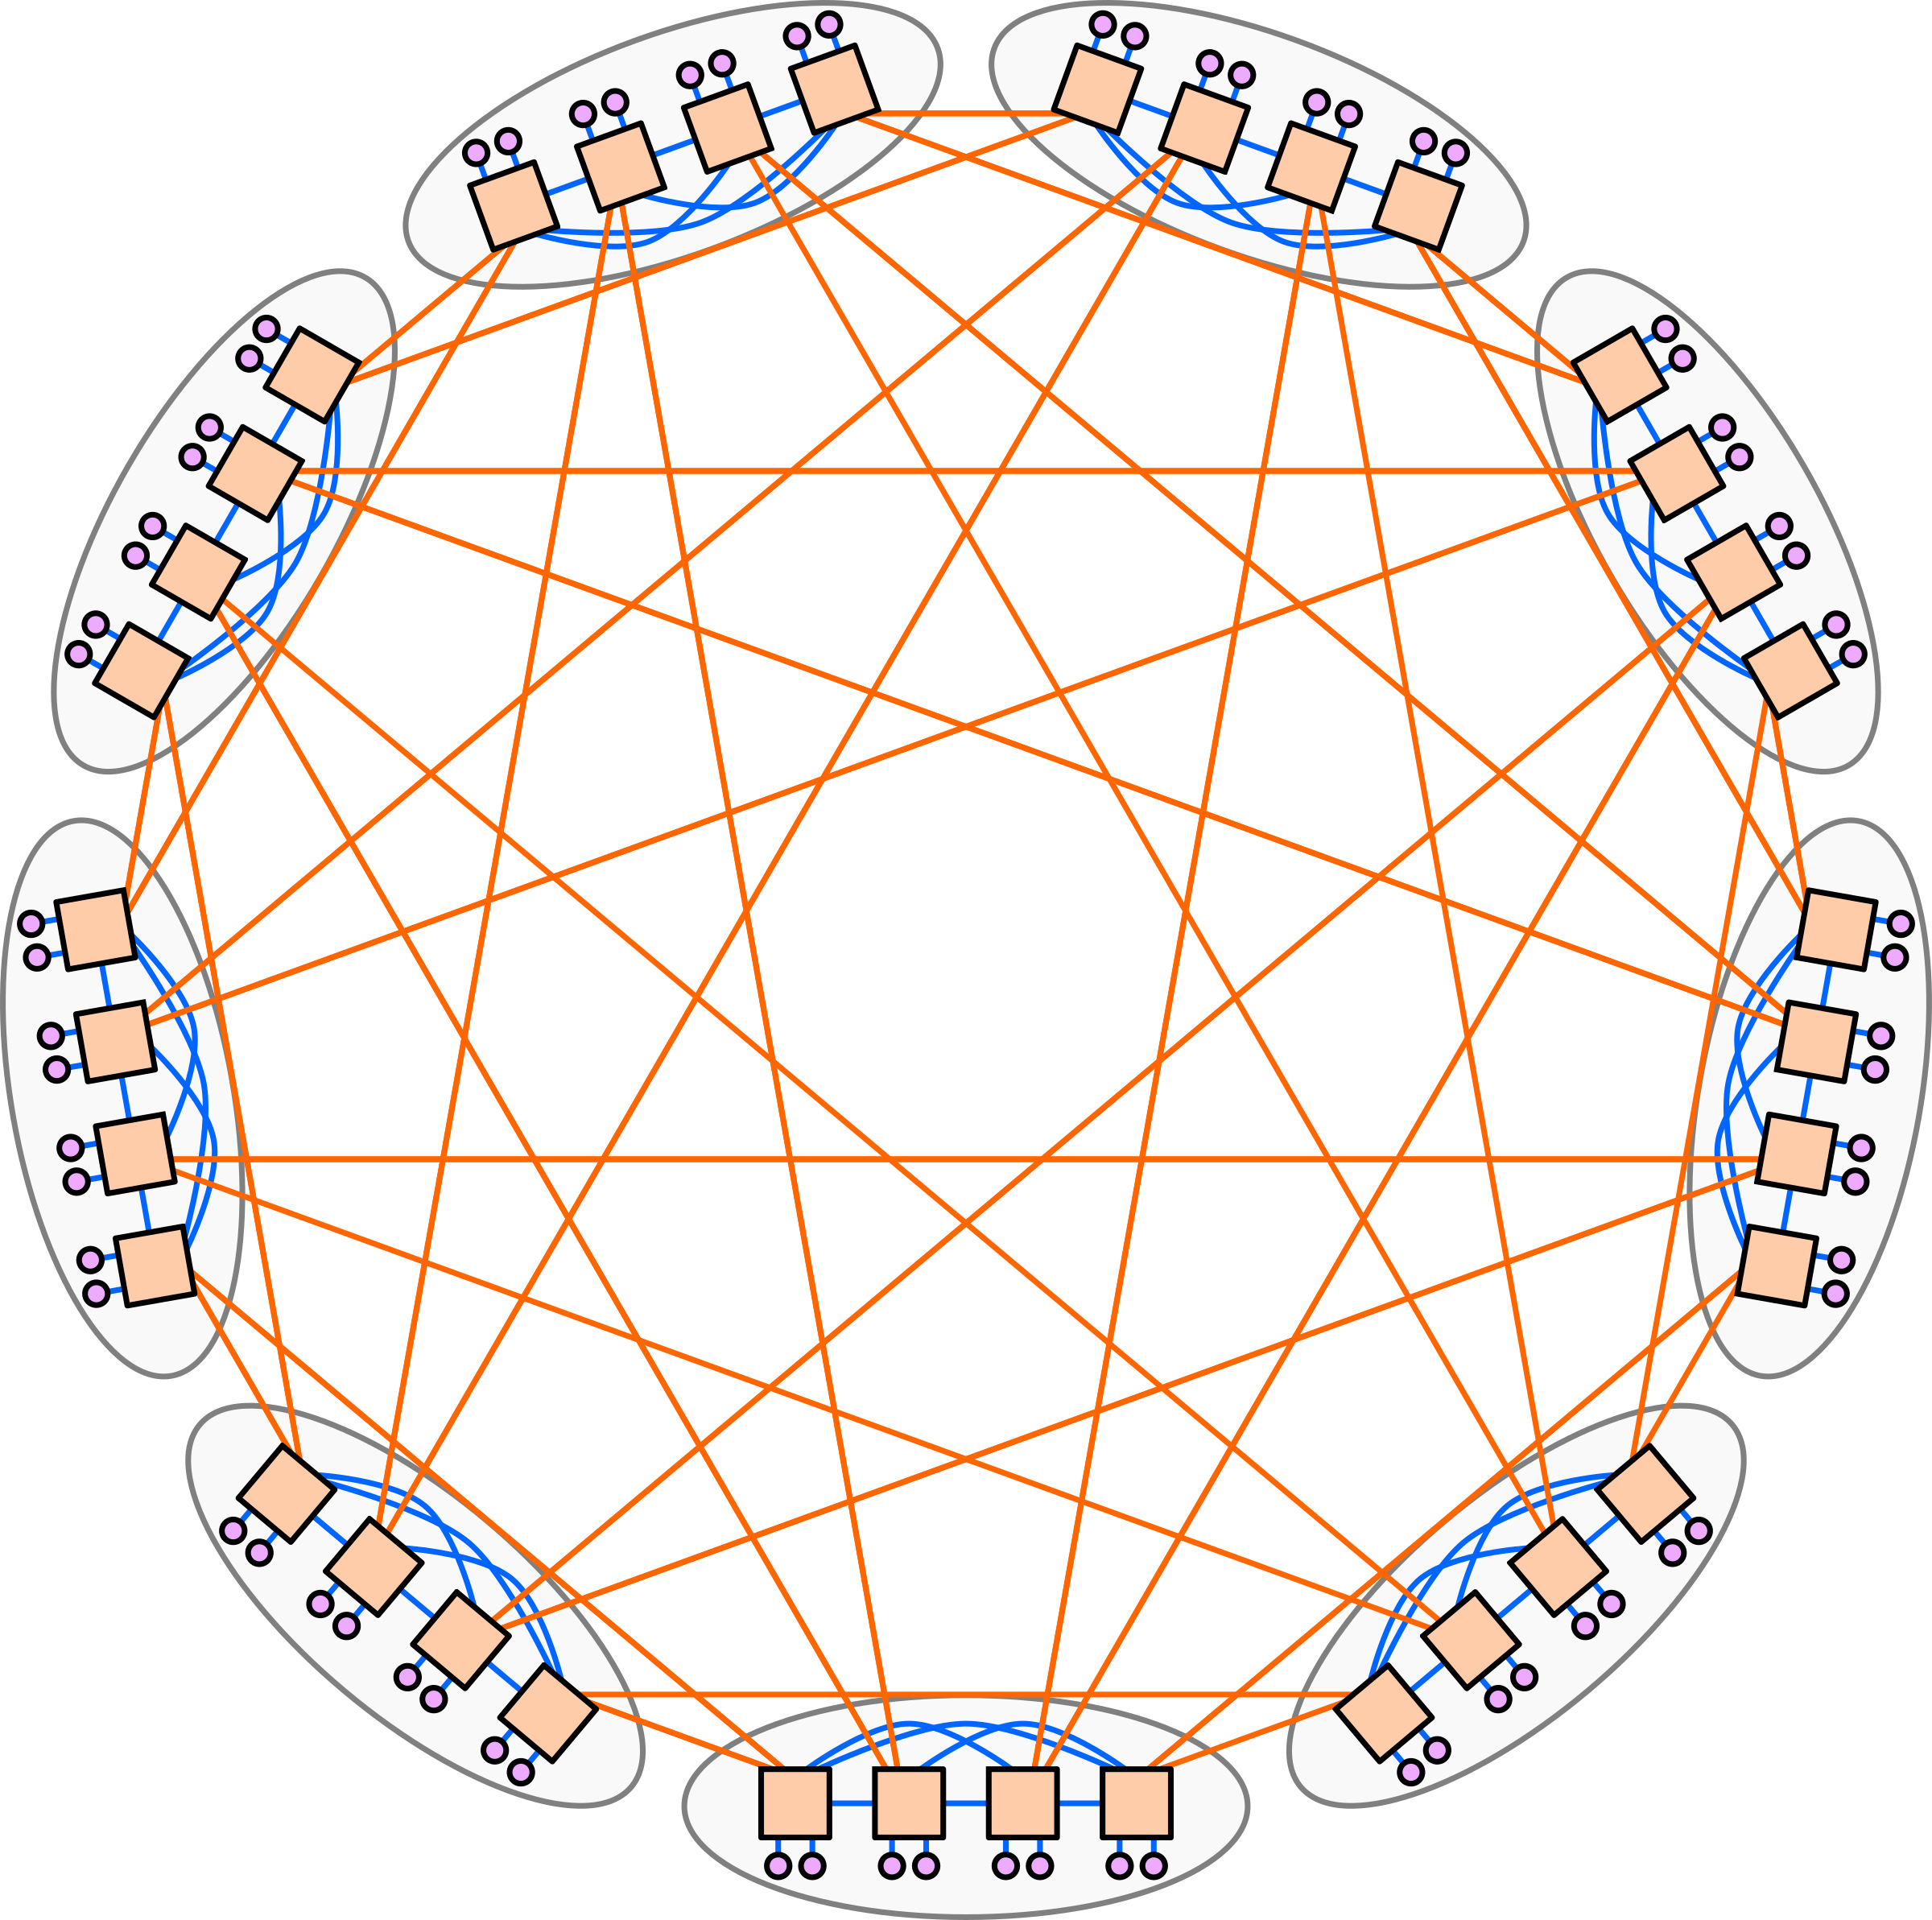
\includegraphics[width=0.6\textwidth]{dragonfly}
\centering
\caption[Um exemplo de rede \dgfly.]{Um exemplo de rede \dgfly. Roteadores e \links globais em laranja, nós em vermelho e \links locais em azul. Fonte: Openclipart, \url{https://openclipart.org/detail/291507/dragonfly-network-topology}, acessado em 08 nov. 2018}
\label{fig:dgfly}
\end{figure}

\subsection{Redes \textit{\Dgfly}}
\label{sec:dgfly}

Uma rede \dgfly é uma rede de conexão indireta e hierárquica que busca ser escalável e reduzir o diâmetro, o custo e a latência da rede.
Uma \dgfly geralmente possuí três níveis: um nível de roteamento, um de grupo e um de sistema.
Cada roteador tem conexões com $p$ PEs, $(r - 1)$ canais locais -- para roteadores do mesmo grupo -- e $h$ canais globais -- para roteadores de outros grupos. Um grupo consiste em $r$ roteadores conectados completamente entre si com $rh$ conexões para outros grupos e $rp$ conexões para nós, formando um roteador virtual que consegue alcançar um número maior de grupos quando comparado com um único roteador~\cite{kim:2008}.
Esta mudança permite uma distinção entre \links locais(intra-grupo) e globais(inter-grupo), utilizando cabeamento e distâncias diferentes, gerando uma latência diferente em \links da rede e permitindo uma redução no custo de cabeamento da rede.
A Figura~\ref{fig:dgfly} exemplifica uma rede \dgfly de três níveis com 9 grupos de 4 roteadores, cada um com 2 nós.

Como um grupo inteiro compartilha cada um de seus \links globais diretamente com outro grupo (Exemplo na Figura~\ref{fig:dgfly_bhat}), a contenção e a alocação de tarefas em uma rede \dgfly afeta severamente seu desempenho.
Para isto uma politica adequada de roteamento, de alocação de tarefas, de migração de tarefas e de carga de trabalho paralela é crucial~\cite{dragonfly}. 
Roteamento dinâmico e adaptativo é um exemplo de política geralmente acoplado a redes \dgfly, para que decisões de roteamento levem em consideração a atual contenção da rede. 
Com isso, caminhos menos sobrecarregados são tomados, distribuindo melhor a carga da rede e evitando problemas graves de contenção~\cite{kim:2008}. 
Balanceamento de carga ciente de topologia também se torna um fator relevante para este tipo de rede.

\begin{figure} [h]
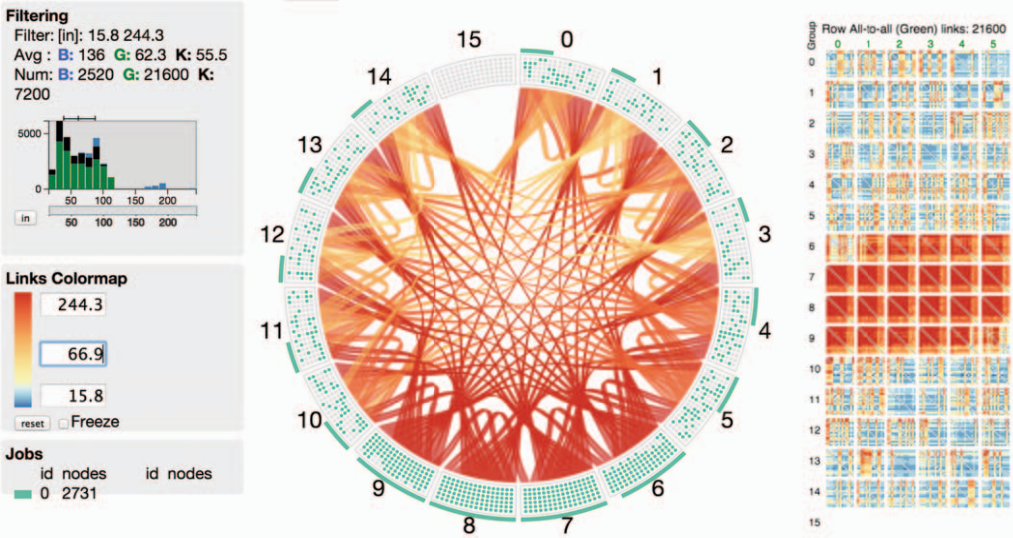
\includegraphics[width=0.8\textwidth]{dgfly_bhat}
\centering
\caption[Exemplo de rede \dgfly de três níveis com 64000 nós em execução, onde 2731 estão alocados para uma tarefa]{Exemplo de rede \dgfly de três níveis com 64000 nós em execução, onde 2731 estão alocados para uma tarefa. \Links globais apresentados no meio e links locais na matriz a direita. Quanto mais avermelhado, mais tráfego na rede~\cite{dragonfly}.}
\label{fig:dgfly_bhat}
\end{figure}


\section{Balanceamento de carga}
\label{sec:lb}

Balanceamento de carga é uma técnica de distribuição de tarefas de maneira que nenhum processador seja sobrecarregado e que reduza custos de comunicação~\cite{Becker}. 
Tendo em vista uma aplicação dinâmica, a distribuição de carga e comunicação se altera ao longo da aplicação, sendo necessário realizar um balanceamento de carga periodicamente para mitigar o desbalanceamento. 

Encontrar um mapeamento ótimo para uma aplicação é um problema NP-\textit{hard}~\cite{leung}. 
Como o objetivo de um balanceamento é aumentar o desempenho, utilizam-se heurísticas para realizar um balanceamento sub-ótimo, já que um mapeamento ótimo iria demorar a ponto de degradar o tempo da aplicação~\cite{pilla-thesis}.

Um \textit{Load Balancer} (LB) pode administrar informações sobre a distribuição de carga e comunicação de três maneiras: Centralizada, Distribuída e Hierárquica.
Um LB centralizado administra a informação do sistema como um todo, podendo realizar decisões mais completas, mas realizando um gargalo de informações. 
Um LB distribuído é o outro extremo, observa somente informações locais, tendo um processo de balanceamento mais escalável, mais rápido porem menos efetivo. 
Uma abordagem hierárquica mistura as duas outras abordagens em camadas hierárquicas diferentes~\cite{Becker}.

Um balanceamento de carga pode utilizar informações da topologia da rede para posicionar tarefas que se comunicam próximas uma da outra, reduzindo a latência de comunicação e efeitos de contenção na rede.
Esta informação se torna ainda mais relevante quando o diâmetro de uma rede é grande, esta possui assimetria ou possui latências diferentes para partes diferentes da rede.
Um LB que utiliza estas informações é dito ciente de topologia.

\subsection{Charm++}
\label{sec:charm}

\charm ~\cite{website:CHARM} é um sistema de programação paralela independente de máquina baseado em C++ e desenvolvido na ~\textit{University of Illinois at Urbana-Champaign} ~\cite{Kale:charm}. 
O sistema é baseado na ideia de objetos migráveis chamado de \chares cuja execução é guiada pela troca de mensagens. 
O seu sistema de execução (\textit{runtime}) possibilita a execução de programas paralelos com mecanismos avançados, como balanceamento de carga automático e \textit{checkpointing}. 
\charm suporta tanto ambientes de multiprocessadores quanto de multicomputadores, conseguindo realizar comunicação através de memória compartilhada e de protocolos ou de infraestruturas de comunicação em rede, tais como UDP, MPI, OFI, Infiniband, uGNI e PAMI~\cite{pilla:CHARM}.

\Chares são objetos concorrentes utilizados no \fw \xspace \charm que possuem somente métodos de entrada visíveis, que são utilizados de maneira remota e assíncrona~\cite{Kale:charm}.
Com estes métodos, \chares podem ser comunicados remotamente sem necessidade de barreiras. Pela sua natureza desacoplável, \chares são altamente migráveis, podendo trocar de PEs com facilidade. 

Para garantir a eficiência na troca de mensagens entre suas tarefas, a plataforma \charm adquire as informações de topologia da rede com o seu \textit{runtime}.
No inicio da execução de uma aplicação, é realizado uma troca de mensagens entre os processos em execução em busca de suas conexões.
Esta informação é utilizada para inferir a topologia utilizada dentre a seguinte lista: \textit{mesh}, \fatt, torus, anel e grafo completo. 


\section{Conclusão}
Em ambientes paralelos e distribuídos informações da topologia podem ser utilizadas para melhorar o desempenho das aplicações.
Alocação de tarefas é uma das técnicas que se beneficia disto, podendo reduzir a latência de comunicação e a contenção de uma rede através de alocação próxima de tarefas que se comuniquem.
Estes fatores se tornam mais impactantes quando se considera redes indiretas e com custos de comunicação diferenciados entre partes da rede.

A plataforma \charm provê um ambiente para programação paralela, criação e uso de balanceadores de carga porém o uso das informações topológicas adquiridas pela plataforma é complexo.
O próximo capítulo aborda a proposta deste trabalho, que visa facilitar o acesso de algumas informações de topologia.


% ----------------------------------------------------------
% Parte de proposta do projeto
% ----------------------------------------------------------


% ---
% Capitulo de Proposta
% ---

\chapter{Proposta}

O objetivo deste trabalho é criar uma abstração da topologia de rede para facilitar o acesso a informações de rede para balanceadores de cargas e outras aplicações.
A utilização desta abstração facilitará a implementação de técnicas que utilizem da topologia para melhorarem seu desempenho.
Na Seção~\ref{sec:trabalhos} são abordados trabalhos que têm intuito similar, na Seção~\ref{sec:requisitos} são estabelecidos os requisitos da abstração, na Seção~\ref{sec:estruturas} são analisados algumas estruturas para a implementação do projeto, na Seção~\ref{sec:my_lb} será apresentado o balanceador que será ajustado e na Seção~\ref{sec:cronograma} é apresentado o cronograma do trabalho.
Neste capítulo serão abordados os requisitos da abstração, as estruturas cogitadas e o cronograma do projeto.


\section{Trabalhos Relacionados}
\label{sec:trabalhos}

Nesta seção são abordados dois trabalhos que abstraem informações de topologia para seu uso em aplicações: O \textit{Portable Hardware Locality} (\hwloc) e o \textit{Portable Network Locality} (\netloc).

\subsection{\Hwloc}

\Hwloc é um software que provê uma abstração da hierarquia das arquiteturas de máquinas, dispondo uma série de informações de cache, núcleos, \textit{multithreading}, \textit{sockets} e dispositivos de entrada e saída~\cite{broquedis:hwloc}.
Seu objetivo é facilitar o acesso de informações complexas das arquiteturas atuais, de maneira uniforme e portável para aplicações. 

Em questão de topologia, o \hwloc trabalha somente em um ambiente multiprocessado, em uma única máquina, não oferecendo suporte em relação a topologia de um ambiente multicomputado ou distribuído.

\subsection{\Netloc}

\Netloc é um projeto de software acoplado ao \hwloc que provê uma abstração da topologia de rede.
Assim como o \hwloc, o software é usado para encontrar informações completas da topologia, ainda não descobertas, e disponibilizar elas para o usuário.
O trabalho do \netloc é voltado para métodos de descobrimento e representação da topologia de rede, unindo estas informações com as informações de máquina do \hwloc~\cite{Goglin:netloc}.

O projeto \netloc ainda está em desenvolvimento e ainda não possui representação de distância ou latência entre pedaços destintos da rede.
Além disso, sua preocupação é de fornecer todas as informações que conseguir sobre a topologia utilizada, de maneira dinâmica para considerar alterações na rede devido a falhas e expansões~\cite{Goglin:netloc}.
Esta carga de informação acoplada ao uso do \hwloc acaba consumindo muita memória de armazenamento e torna lento o acesso das informações armazenadas.
A lentidão de acesso adiciona um custo indesejado a um balanceador de carga, que deve ser executado em um espaço curto de tempo para que o tempo total da aplicação seja reduzida.


\section{Requisitos}
\label{sec:requisitos}

Os requisitos da abstração são os seguintes:

\begin{itemize}
    \item A abstração deverá ser capaz de fornecer a distância entre PEs dentro da rede, fornecendo a latência de comunicação ou a proximidade entre PEs, de modo que esta possa ser utilizada em um balanceador de carga.
    \item A utilização da abstração deve ser simples e com pouco sobrecusto, facilitando o desenvolvimento de balanceadores sem debilitar seu desempenho.
    \item A estrutura criada para a abstração da topologia deve poder ser armazenada, para que não tenha de ser descoberta ou inicializada novamente no mesmo sistema.
    \item A abstração construída deve ser compatível com a plataforma \charm, para ser utilizado em seu módulo de balanceamento de carga.
\end{itemize}
%especificar mais, razão das coisas
% Tente abordar aqui coisas como hwloc e netloc como inspiração também. Lembre de trazer como requisito a fácil usabilidade e funcionamento com o Charm++
% salvar e carregar topologias?

\section{Estrutura}
\label{sec:estruturas}

Existem diversas maneiras de representar uma estrutura de grafo, e seus benefícios são dependentes de como a estrutura é utilizada.
Foi cogitado três abordagens possíveis para o que será armazenado: um armazenamento de distâncias, um armazenamento da estrutura geral da topologia ou ambos.
A primeira têm acesso mais rápido e ocupa menos memória pois armazena menos informação mas é menos completa que a segunda, barrando utilidades futuras.
A terceira opção consiste no uso de ambas as estruturas, gerando maior ocupação de memória mas obtendo os benefícios de ambas. 

Quatro estruturas são avaliadas para a representação da topologia, observando suas vantagens, desvantagens e aplicabilidade para este projeto.
Na Tabela~\ref{tab:struct_comparison} é observada a complexidade do tempo de acesso a uma ligação específica da estrutura, de tamanho ocupado na memória e de inserção de uma ligação, todos em relação ao número de nós $p$, ao número de arestas $l$ e ao grau $g$ da topologia. As estruturas são descritas a seguir.

\begin{itemize}
    \item \textbf{Lista de listas}: Uma representação que dispõe os nós da topologia em uma lista e cada nó possui uma lista de suas ligações. 
    É uma estrutura simples que têm tempo de acesso dependente do número de nós e do número máximo de arestas em cada nó.
    Ocupa memória de acordo com o número de nós e o número de arestas.
    Esta estrutura é utilizada no módulo de balanceamento de carga do \charm.

    \item \textbf{Árvore}: Uma árvore representando uma hierarquia de proximidade. 
    Tem acesso logaritmo relativo ao número de nós e ocupa memória linearmente em relação ao número de nós. 
    É utilizada no \hwloc para a estrutura topológica interna de uma máquina. 
    No \hwloc os PEs se encontram como folhas da árvore e são agrupados de acordo com a proximidade dentro da máquina.
    Esta abordagem se adequa bem para topologia interna devido a sua hierarquia inerente, mas não descreve bem uma topologia não hierárquica, como uma torus, pois muitas máquinas se encontram no mesmo nível hierárquico e possuem arestas entre si.
    Uma árvore não tem inserção de ligação e encontra a distâncias entre dois pontos através de dois acessos a árvore.

    \item \textbf{Matriz}: Uma matriz representando todas as associações possíveis entre os nós da rede.
    Tem tempo constante de acesso a uma ligação mas ocupa memória quadrática em relação ao número de nós.
    Uma das vantagens de uma matriz é sua alta mutabilidade de ligações, sendo possível alteração ou inserção posteriores de ligações na topologia com tempo constante.

    \item \textbf{\textit{Compressed Sparse Columns}} (CSC): uma representação construída a partir de uma matriz, retirando todas as ligações inexistentes para economia de memória.
    A estrutura é organizada em três listas: uma lista com os valores não nulos da matriz, uma lista com as linhas destes valores e uma lista que indexa o início das linhas de cada coluna.
    Utiliza índices de acesso similar a uma lista de listas.
    É feita de maneira a otimizar localidade temporal de memoria quando é realizado uma travessia do grafo~\cite{sun:csr}.
    O problema de uma CSC é sua baixa mutabilidade, necessitando uma refatoração para inserir novas arestas ou de um número de espaços vazios na sua inicialização, que podem não ser o suficiente.
\end{itemize}

\setlength{\tabcolsep}{0.5em}
\begin{table}[!ht]
    \centering
    \begin{tabular}{l c c c}
        \toprule
        \textbf{Estrutura} & \textbf{Acesso} &  \textbf{Memória utilizada} & \textbf{Inserção de ligação} \\ \midrule
        %\hline
        Listas de Listas & $O(g)$ & $O(p \times g)$ & $O(2g)$ \\
        Matriz & $O(1)$ & $O(p^2)$ & $O(1)$ \\
        Árvore & $O(log_f p)$ & $O(p)$ & $*$ \\
        CSC &  $O(g)$ & $O(p+l)$ & $O(p + l)$  \\ \bottomrule
    \end{tabular}
    \caption[Complexidade de acesso e de memória das estruturas cogitadas.]{Complexidade de acesso e de memória das estruturas cogitadas.}
    \label{tab:struct_comparison}
\end{table}


Uma estrutura puramente topológica não proveria um acesso rápido para distância pois teria de calculá-la a cada chamada.
Uma estrutura somente de distâncias se usada como um mecanismo de memoização, em algum momento se tornaria um grafo completo, onde $g = l = p$. 
Quando isto ocorrer, todas as estruturas apresentadas ocupariam memória quadrática em relação ao número de PEs, exceto uma árvore, que não oferece um acesso constante à distância. 
Esta abordagem não escalaria com o número de PEs. Realizar uma abordagem com ambas as estruturas resultaria num uso extenso da memória, algo indesejável para uma aplicação distribuída e escalável.

Para alcançar escalabilidade, será utilizada uma estrutura inspirada no \netloc, dividindo a topologia em dois níveis: uma camada hierárquica em árvore que representa a topologia interna das máquinas, similar ao \hwloc, e outra camada que apresenta as conexões em um nível de rede, representada com CSC pela sua utilidade em travessia de grafos. 
Uma matriz de distâncias será utilizada como mecanismo de memoização para distâncias no nível de rede, reduzindo seu tamanho por considerar somente um nível de hierarquia. Além disto, será assumido simetria no nível de rede, possibilitando a compressão desta matriz.

A Figura~\ref{fig:estru} apresenta as estruturas propostas para representar a topologia da Imagem~\ref{fig:estru:topo}, os PEs então em azul, as máquinas em vermelho e as distâncias. 
A Imagem~\ref{fig:estru:arvore} apresenta a estrutura hierárquica de árvore das máquinas desta topologia e a tabela \ref{fig:estru:csc} a representação das distâncias das máquinas com CSC. 
A estrutura matricial para memoização das distâncias entre máquinas é representada pela tabela~\ref{fig:estru:matriz} representa a estrutura matricial proposta para a memoização de distâncias entre as máquinas, onde a primeira linha e primeira coluna indicam os nós de máquina e as cédulas internas representam as distâncias.
Um 'X' indica que a posição não é armazenada para economia de memória e um espaço em branco indica uma distância ainda não calculada.

\begin{figure}[h]
\begin{subfigure}{.5\textwidth}
    \centering
    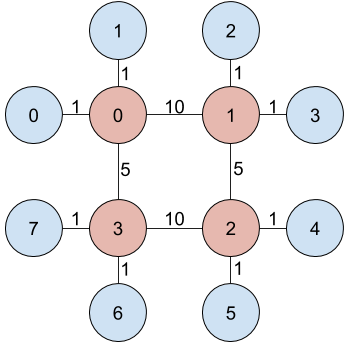
\includegraphics[width=0.8\linewidth]{images/estrutura_abst_topo.png}
    \caption{Topologia}
    \label{fig:estru:topo}
\end{subfigure}
\begin{subfigure}{.5\textwidth}
    \centering
    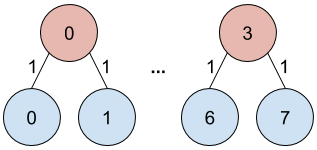
\includegraphics[width=0.8\linewidth]{images/estrutura_abst_arvore.png}
    \caption{Árvore}
    \label{fig:estru:arvore}
\end{subfigure}
\begin{subfigure}{.5\textwidth}
    \centering
    \begin{tabular}{|l|c|c|c|c|c|c|c|c|}
        \cline{1-6}
        Índice     & 0 & 2  & 4 & 5 & 8  \\ \hline
        Linha      & 1 & 3 & 0 & 2 & 1 & 3 & 0 & 2  \\ \hline
        Distância  & 10 & 5 & 10 & 5 & 5 & 10 & 5 & 10 \\ \hline
    \end{tabular}
    \caption{CSC}
    \label{fig:estru:csc}
\end{subfigure}
\begin{subfigure}{.5\textwidth}
    \centering
    \begin{tabular}{|c|c|c|c|c|}
        \hline
         M & 0 & 1  & 2 & 3  \\ \hline
         0 & X & 10 &   & 5  \\ \hline
         1 & X & X  & 5 & 15 \\ \hline
         2 & X & X  & X & 10  \\ \hline
         3 & X & X  & X & X  \\ \hline
    \end{tabular}
    \caption{Matriz}
    \label{fig:estru:matriz}
\end{subfigure}
\caption[Representação das estruturas utilizadas.]{Representação da topologia da imagem (a) seguindo as estruturas propostas.}
\label{fig:estru}
\end{figure}

Nesta estrutura a complexidade de acesso de uma distância qualquer será de $O(g)$ e de $O(1)$ caso tenha sido calculada anteriormente.
Sendo $c$ a média do número de PEs por máquinas e $m$ o número de máquinas, o uso de memória será de $O(mc)$ para as estruturas de árvore, de $\frac{p+l}{c}$ para o CSC e de $\frac{p^2}{2c^2}$ para a matriz de memoização.
%O custo de criação da estrutura será dependente do número de PEs na rede e do tempo de acesso e descobrimento da informações topológicas usadas de base, como o do \runtime \charm.

%complexidade de montar estrutura (diferença entre computacional e procura), complexidades

\section{Balanceador de Carga}
\label{sec:my_lb}

Para a demonstração do funcionamento da abstração da topologia de rede, será modificado um balanceador de carga distribuído presente na plataforma \charm, de nome NeighborLB.
Este balanceador observa somente PEs vizinhos para a tomada de decisão de balanceamento, evitando contenção da rede e obtendo baixa latência nas mensagens.
Assim como outros balanceadores distribuídos, é escalável pois independe do número de nós da rede, mas seu balanceamento é limitado pela quantidade de informação.

O descobrimento de vizinhos no balanceador NeighborLB é dado através de um balanceador base que existe dentro da plataforma \charm que utiliza seu mecanismo de inferência.
Este mecanismo será substituído pela abstração criada para comprovar seu funcionamento.

%mas eu vou tirar informação do charm pra por de novo? > facilidade no acesso, sem ter de realizar de novo


\section{Cronograma}
\label{sec:cronograma}

As atividades previstas no projeto estão descritas abaixo:

\begin{itemize}
	\item \textbf{A1: Implementação da abstração da topologia de rede.} Nesta parte do trabalho será implementado as estruturas e algoritmos para o funcionamento da abstração.
	\item \textbf{A2: Desenvolvimento de uma interface da abstração de topologia utilizando a plataforma \charm.} A abstração será complementada com uma interface utilizando \charm.
	\item \textbf{A3: Ajuste de um balanceador de carga para a prova de conceito.} Nesta etapa será modificado o balanceador de carga NeighborLB para que utilize a abstração utilizada, comprovando o funcionamento desta.
	\item \textbf{A4: Escrita do rascunho do TCC II.} A escrita do rascunho do TCC II será realizada neste período. A entrega deste documento está prevista para a segunda semana do mês de maio.
	\item \textbf{A5: Preparação da defesa pública.} Nesta etapa será realizada a preparação da apresentação oral e visual do conteúdo deste trabalho para a defesa pública.
	\item \textbf{A6: Defesa pública.} Nesta etapa será realizada a defesa do projeto desenvolvido. Pretende-se realizar a defesa pública do trabalho na primeira semana do mês de junho.
	\item \textbf{A7: Correções e entrega da versão final do TCC.} Nesta etapa serão realizadas as correções e os ajustes da monografia e a entrega final do documento. A entrega da versão final está prevista para a quarta semana do mês de junho.
\end{itemize}

A Figura~\ref{fig:cronograma} apresenta o cronograma previsto para a realização das atividades descritas anteriormente. As atividades estão distribuídas ao longo do fim de 2018 e o primeiro semestre de 2019.

% \begin{adjustwidth}{-2.5cm}{}
  \begin{figure}[h]
    \begin{center}
     \begin{ganttchart}[
       y unit title=0.4cm,
       y unit chart=0.6cm,
       hgrid,
       vgrid={{dotted, dotted, dotted, black}},
       title label font=\scriptsize,
       title/.append style={fill=gray!30},
       title height=1,
       bar/.append style={fill=gray!30,rounded corners=2pt},
       bar label font=\scriptsize,
       group label font=\scriptsize,
     ]{1}{28}
     	\gantttitle{\textbf{2018}}{4}
	 \gantttitle{\textbf{2019}}{24}\\
		\gantttitle{\textbf{Dez}}{4}
     \gantttitle{\textbf{Jan}}{4}
	 \gantttitle{\textbf{Fev}}{4}
	 \gantttitle{\textbf{Mar}}{4}
	 \gantttitle{\textbf{Abr}}{4}
	 \gantttitle{\textbf{Mai}}{4}
	 \gantttitle{\textbf{Jun}}{4
}\\

     \ganttbar{A1}{1}{7} \\
     \ganttbar{A2}{7}{14} \\
     \ganttbar{A3}{15}{16} \\
     \ganttbar{A4}{17}{22} \\
     \ganttbar{A5}{23}{26} \\
     \ganttbar{A6}{26}{26} \\
     \ganttbar{A7}{27}{28}
     \end{ganttchart}
%  \end{adjustwidth}
     \caption{Cronograma de atividades.}\label{fig:cronograma}
  \end{center}
\end{figure}
% ---


% 
\def\coordenador{Renato Cislaghi}
\def\orientador{Vinicius Marino Calvo Torres de Freitas}
\def\coorientador{Márcio Bastos Castro}
\def\autor{Thales Alexandre Zirbel Hubner}


\chapter{Planejamento}

Este capítulo contém o planejamento do projeto onde cada parte do plano de gerenciamento se encontra em seções diferentes. A Seção \ref{sec:cronograma} apresenta as atividades planejadas e seu cronograma a ser seguido ao longo da realização deste trabalho. A Seção \ref{sec:rh} apresenta os recursos humanos envolvidos. A Seção \ref{sec:custos} indica os custos estimados para a execução do projeto. A Seção \ref{sec:comunicacao} dispõe o gerenciamento da comunicação entre as partes envolvidas. A Seção \ref{sec:riscos} apresenta os riscos identificados e suas respectivas estratégias.

% ---
\section{Cronograma}
%\label{sec:cronograma}

As atividades previstas no projeto estão descritas abaixo:

\begin{itemize}
	\item \textbf{A1: Estudo da fundamentação teórica.} Nesta parte inicial será realizada a revisão de artigos e materiais relacionados a computação paralela, topologia de rede e balanceamento de carga.
	\item \textbf{A2: Familiarização com a plataforma charm++.} Processo de familiarização com a plataforma para programação paralela a ser utilizada.
	\item \textbf{A3: Revisão do estado da arte e prática.} Nesta etapa será tratada a revisão do estado da arte envolvido no contexto do trabalho, a fim de  fortalecer a base do conhecimento necessária para a realização do mesmo.
	\item \textbf{A4: Elaboração da proposta.} Nesta etapa será apresentada a proposta de solução do problema em questão, bem como suas estratégias de implementação.
	\item \textbf{A5: Escrita do relatório do TCC I.} Nesta etapa será realizada a escrita do relatório do TCC I. A entrega deste documento está prevista para a quarta semana do mês de novembro.
	\item \textbf{A6: Implementação da abstração da topologia de rede.} Nesta parcela será realizada a implementação da abstração proposta assim como a verificação do funcionamento desta.
	\item \textbf{A7: Teste da abstração da topologia de rede.} Nesta parcela será realizada a verificação do funcionamento da abstração.
	\item \textbf{A8: Desenvolvimento de um balanceador de carga.} Nesta etapa será efetuada o desenvolvimento de um balanceador de carga que utilize a abstração de rede criada.
	\item \textbf{A9: Testes e comparações de desempenho.} Nesta etapa será efetuado testes de desempenho do balanceador de carga a a comparação deste com outros balanceadores existentes.
	\item \textbf{A10: Escrita do rascunho do TCC II.} A escrita do rascunho do TCC II será realizada neste período. A entrega deste documento está prevista para a segunda semana do mês de maio.
	\item \textbf{A11: Preparação da defesa pública.} Nesta etapa será realizada a preparação da apresentação oral e visual do conteúdo deste trabalho para a defesa pública.
	\item \textbf{A12: Defesa pública.} Nesta etapa será realizada a defesa do projeto desenvolvido. Pretende-se realizar a defesa pública do trabalho na primeira semana do mês de junho.
	\item \textbf{A13: Correções e entrega da versão final do TCC.} Nesta etapa serão realizadas as correções e os ajustes da monografia e a entrega final do documento. A entrega da versão final está prevista para a quarta semana do mês de junho.
\end{itemize}

A Figura~\ref{fig:cronograma} apresenta o cronograma previsto para a realização das atividades descritas anteriormente. As atividades estão distribuídas ao longo do primeiro e segundo semestres de 2018 e o primeiro semestre de 2019.

% \begin{adjustwidth}{-2.5cm}{}
  \begin{figure}[h]
    \begin{center}
     \begin{ganttchart}[
       y unit title=0.4cm,
       y unit chart=0.6cm,
       hgrid,
       vgrid={{dotted, dotted, dotted, black}},
       title label font=\scriptsize,
       title/.append style={fill=gray!30},
       title height=1,
       bar/.append style={fill=gray!30,rounded corners=2pt},
       bar label font=\scriptsize,
       group label font=\scriptsize,
     ]{1}{30}
     	\gantttitle{\textbf{2018}}{18}
	 \gantttitle{\textbf{2019}}{12}\\
	 	\gantttitle{\textbf{Abr}}{2}
	 	\gantttitle{\textbf{Mai}}{2}
	 	\gantttitle{\textbf{Jun}}{2}
	 	\gantttitle{\textbf{Jul}}{2}
	 	\gantttitle{\textbf{Ago}}{2}
	 	\gantttitle{\textbf{Set}}{2}
	 	\gantttitle{\textbf{Out}}{2}
		\gantttitle{\textbf{Nov}}{2}						\gantttitle{\textbf{Dez}}{2}
     \gantttitle{\textbf{Jan}}{2}
	 \gantttitle{\textbf{Fev}}{2}
	 \gantttitle{\textbf{Mar}}{2}
	 \gantttitle{\textbf{Abr}}{2}
	 \gantttitle{\textbf{Mai}}{2}
	 \gantttitle{\textbf{Jun}}{2
}\\
     
     \ganttbar{A1}{1}{6} \\
     \ganttbar{A2}{2}{8} \\
     \ganttbar{A3}{5}{7} \\
     \ganttbar{A4}{5}{7} \\
     \ganttbar{A5}{9}{16} \\
     \ganttbar{A6}{9}{14} \\
     \ganttbar{A7}{14}{16} \\
     \ganttbar{A8}{16}{22} \\
     \ganttbar{A9}{22}{26} \\
     \ganttbar{A10}{24}{27} \\
     \ganttbar{A11}{26}{29} \\
     \ganttbar{A12}{29}{29} \\
     \ganttbar{A13}{29}{30}
     \end{ganttchart}
%  \end{adjustwidth}
     \caption{Cronograma de atividades.}%\label{fig:cronograma}
  \end{center}
\end{figure}
% ---
\begin{comment} 
\section{Cronograma}
\label{sec:cronograma}

As atividades previstas no projeto estão descritas abaixo:

\begin{itemize}
	\item \textbf{A1: Implementação da abstração da topologia de rede.} Nesta parte do trabalho será implementado as estruturas e algoritmos para o funcionamento da abstração.
	\item \textbf{A2: Desenvolvimento de uma interface da abstração de topologia utilizando a plataforma \charm.} A abstração será complementada com uma interface utilizando \charm.
	\item \textbf{A3: Ajuste de um balanceador de carga para a prova de conceito.} Nesta etapa será modificado o balanceador de carga NeighborLB para que utilize a abstração utilizada, comprovando o funcionamento desta.
	\item \textbf{A4: Escrita do rascunho do TCC II.} A escrita do rascunho do TCC II será realizada neste período. A entrega deste documento está prevista para a segunda semana do mês de maio.
	\item \textbf{A5: Preparação da defesa pública.} Nesta etapa será realizada a preparação da apresentação oral e visual do conteúdo deste trabalho para a defesa pública.
	\item \textbf{A6: Defesa pública.} Nesta etapa será realizada a defesa do projeto desenvolvido. Pretende-se realizar a defesa pública do trabalho na primeira semana do mês de junho.
	\item \textbf{A7: Correções e entrega da versão final do TCC.} Nesta etapa serão realizadas as correções e os ajustes da monografia e a entrega final do documento. A entrega da versão final está prevista para a quarta semana do mês de junho.
\end{itemize}

A Figura~\ref{fig:cronograma} apresenta o cronograma previsto para a realização das atividades descritas anteriormente. As atividades estão distribuídas ao longo do fim de 2018 e o primeiro semestre de 2019.

% \begin{adjustwidth}{-2.5cm}{}
  \begin{figure}[h]
    \begin{center}
     \begin{ganttchart}[
       y unit title=0.4cm,
       y unit chart=0.6cm,
       hgrid,
       vgrid={{dotted, dotted, dotted, black}},
       title label font=\scriptsize,
       title/.append style={fill=gray!30},
       title height=1,
       bar/.append style={fill=gray!30,rounded corners=2pt},
       bar label font=\scriptsize,
       group label font=\scriptsize,
     ]{1}{28}
     	\gantttitle{\textbf{2018}}{4}
	 \gantttitle{\textbf{2019}}{24}\\
		\gantttitle{\textbf{Dez}}{4}
     \gantttitle{\textbf{Jan}}{4}
	 \gantttitle{\textbf{Fev}}{4}
	 \gantttitle{\textbf{Mar}}{4}
	 \gantttitle{\textbf{Abr}}{4}
	 \gantttitle{\textbf{Mai}}{4}
	 \gantttitle{\textbf{Jun}}{4
}\\

     \ganttbar{A1}{1}{7} \\
     \ganttbar{A2}{7}{14} \\
     \ganttbar{A3}{15}{16} \\
     \ganttbar{A4}{17}{22} \\
     \ganttbar{A5}{23}{26} \\
     \ganttbar{A6}{26}{26} \\
     \ganttbar{A7}{27}{28}
     \end{ganttchart}
%  \end{adjustwidth}
     \caption{Cronograma de atividades.}\label{fig:cronograma}
  \end{center}
\end{figure}

\end{comment}

% ---
\section{Recursos Humanos}
\label{sec:rh}
\begin{center}
\begin{tabular}{|c|c|}
\hline
    Papel & Nome \\ \hline
    Orientador & \orientador \\ \hline
    Coorientador & \coorientador \\ \hline
    Coordenador & \coordenador \\ \hline
    Membro da Banca I & \\ \hline
    Membro da Banca II & \\ \hline
    Autor & \autor \\ \hline
\end{tabular}
\end{center}
% ---
% ---
\section{Custos}
\label{sec:custos}

\begin{center}
\begin{tabular}{|c|c|c|c|c|c|}
\hline
\multicolumn{6}{|c|}{Estimativas para Recursos Humanos} \\ \hline
    Nome & Data Início & Data Fim & Hora/Mês & Valor/Hora & Custo Total \\ \hline
    Autor & 01/04/2018 & 01/06/2019 & 40 & R\$ 15,00 & R\$ 8400,00 \\ \hline
    Orientador & 01/04/2018 & 01/06/2019 & 4 & R\$ 20,00 & R\$ 1120,00 \\ \hline
    Coorientador & 01/04/2018 & 01/06/2019 & 4 & R\$ 71,00 & R\$ 3976,00 \\ \hline
    Coordenador & 01/04/2018 & 01/06/2019 & 1 & R\$ 102,00 & R\$ 1428,00 \\ \hline
    Membro da Banca I & 01/05/2019 & 01/06/2019 & 1 & R\$ 60,00 & R\$ 60,00 \\ \hline
    Membro da Banca II & 01/05/2019 & 01/06/2019 & 1 & R\$ 60,00 & R\$ 60,00 \\ \hline
\multicolumn{5}{|l|}{Subtotal estimativas para recursos humanos} & R\$ 15044,00 \\
\hline
\end{tabular}
\end{center}

\begin{center}
\resizebox{\textwidth}{!}{
    \begin{tabular}{|c|c|c|c|c|c|}
    \hline
    \multicolumn{6}{|c|}{Estimativas para Recursos Não Humanos} \\ \hline
        Descrição & Data Início & Data Fim & Quantidade & Valor Unitário & Custo Total \\
        \hline
        Computador para uso & 04/18 & 06/19 & 1 & R\$ 2500,00 & R\$ 2500,00 \\ \hline
        CDs para o código desenvolvido & 06/19 & 06/19 & 2 & R\$ 4,00 & R\$ 8,00 \\ \hline
        Impressão para o relatório & 12/18 & 12/18 & 3 & R\$ 20,00 & R\$ 60,00 \\ \hline
    \multicolumn{5}{|l|}{Subtotal estimativas para recursos não humanos} & R\$ 2568,00 \\
    \hline
    \end{tabular}
}
\end{center}
% ---

% ---
\section{Comunicação}
\label{sec:comunicacao}

\begin{center}
\begin{tabular}{|l|p{9cm}|}
\hline
    O que precisa ser comunicado & Reuniões periódicas com o Orientador e Coorientador\\ \hline
    Emissor & \autor \\ \hline
    Receptor & \orientador, \coorientador \\ \hline
    Comunicação & Reuniões periódicas com o Orientador para acompanhamento do projeto\\ \hline
    Forma de comunicação & Pessoalmente \\ \hline
    Frequência ou Quando & Quinzenalmente \\ \hline
\end{tabular}
\end{center}

\begin{center}
\begin{tabular}{|l|p{9cm}|}
\hline
    O que precisa ser comunicado & Entrega da Proposta \\ \hline
    Emissor & \autor \\ \hline
    Receptor & \coordenador \\ \hline
    Comunicação & Entrega da proposta completa do TCC \\ \hline
    Forma de comunicação & Sistema de TCC \\ \hline
    Frequência ou Quando & Única vez \\ \hline
\end{tabular}
\end{center}

\begin{center}
\begin{tabular}{|l|p{9cm}|}
\hline
    O que precisa ser comunicado & Entrega do Relatório em TCC I \\ \hline
    Emissor & \autor \\ \hline
    Receptor & \coordenador \\ \hline
    Comunicação & Entrega da primeira parte da monografia \\ \hline
    Forma de comunicação & Sistema de TCC \\ \hline
    Frequência ou Quando & Única vez \\ \hline
\end{tabular}
\end{center}

\begin{center}
\begin{tabular}{|l|p{9cm}|}
\hline
    O que precisa ser comunicado & Entrega da primeira versão da monografia completa em TCC II \\ \hline
    Emissor & \autor \\ \hline
    Receptor & \coordenador \\ \hline
    Comunicação & Entrega da primeira versão da monografia completa \\ \hline
    Forma de comunicação & Sistema de TCC \\ \hline
    Frequência ou Quando & Única vez \\ \hline
\end{tabular}
\end{center}

\begin{center}
\begin{tabular}{|l|p{9cm}|}
\hline
    O que precisa ser comunicado & Defesa do TCC \\ \hline
    Emissor & \autor \\ \hline
    Receptor & \orientador, \coorientador, Membro da Banca I, Membro da Banca II\\ \hline
    Comunicação & Realização da defesa do TCC aos membros da banca.  \\ \hline
    Forma de comunicação & Pessoalmente \\ \hline
    Frequência ou Quando & Única vez \\ \hline
\end{tabular}
\end{center}


\begin{center}
\begin{tabular}{|l|p{9cm}|}
\hline
    O que precisa ser comunicado & Entrega da versão final da monografia \\ \hline
    Emissor & \autor \\ \hline
    Receptor & \coordenador \\ \hline
    Comunicação & Entrega da monografia com os ajustes feitos após a defesa\\ \hline
    Forma de comunicação & Sistema de TCC \\ \hline
    Frequência ou Quando & Única vez \\ \hline
\end{tabular}
\end{center}
% ---

% ---
\newpage
\section{Riscos}
\label{sec:riscos}

\begin{center}
\resizebox{\textwidth}{!}{
    \begin{tabular}{|l|c|c|c|c|l|}
    \hline
        Nome & Probabilidade & Impacto & Exposição & 
        Estratégia & Ações de Prevenção  \\ \hline
        
         \makecell[l]{Perda de arquivos} & Baixa & Alto & Média & Mitigar &\makecell[l]{ Realizar backups \\ com frequencia \\ semanal e utilizar \\ armazenamento \\ em nuvem.}  \\ \hline
         \makecell[l]{Alteração no cronograma} & Baixa & Alto & Média & Aceitar &\makecell[l]{ - }  \\ \hline
         \makecell[l]{Alteração no escopo} & Baixa & Alto & Média & Aceitar &\makecell[l]{ - }  \\ \hline
         \makecell[l]{Problemas de saúde \\ do Orientando} & Média & Baixo & Baixa & Aceitar &\makecell[l]{ - } \\ \hline
         \makecell[l]{Indisponibilidade do \\ Orientador/Coorientador} & Média & Médio & Média & Aceitar & -\\ \hline
         \makecell[l]{Indisponibilidade da \\ plataforma para testes} & Média & Alto & Alta & Mitigar &\makecell[l] {Contato com  \\ responsáveis \\ pela plataforma \\ e agendamento \\ de execuções.} \\ \hline
    \end{tabular}
}
\end{center}

% ---

% ---
% Finaliza a parte no bookmark do PDF, para que se inicie o bookmark na raiz
% ---
\bookmarksetup{startatroot}% 
% ---

% ----------------------------------------------------------
% ELEMENTOS PÓS-TEXTUAIS
% ----------------------------------------------------------
\postextual


% ----------------------------------------------------------
% Referências bibliográficas
% ----------------------------------------------------------

\bibliography{bibliography}


\end{document}
\grid
\grid
